
\documentclass[10pt]{article}

\usepackage[a4paper,margin=0.65in]{geometry}
\usepackage{amsmath,amssymb}
\usepackage{graphicx}
\usepackage{booktabs}
\usepackage{array}
\usepackage{float}
\usepackage[font=small,labelfont=bf,skip=3pt]{caption}
\usepackage{hyperref}
\usepackage{enumitem}
\usepackage{xcolor}
\usepackage{tikz}
\usetikzlibrary{positioning,arrows.meta,shapes.geometric,fit,calc}

\setlist{nosep,leftmargin=*}
\renewcommand{\arraystretch}{1.2}
\setlength{\parindent}{0pt}
\setlength{\parskip}{2pt}
\setlength{\abovedisplayskip}{3pt}
\setlength{\belowdisplayskip}{3pt}
\setlength{\abovedisplayshortskip}{1pt}
\setlength{\belowdisplayshortskip}{2pt}
\graphicspath{{figures/}}

\tikzset{
layer/.style={
draw,
rounded corners,
minimum width=1.7cm,
minimum height=0.65cm,
align=center,
fill=blue!10,
font=\scriptsize
},
smalllayer/.style={
draw,
rounded corners,
minimum width=1.35cm,
minimum height=0.58cm,
align=center,
fill=green!10,
font=\scriptsize
},
arrow/.style={
-{Latex[length=2mm]},
thin
}
}

\begin{document}

%%%%%%%%%%%%%%%%%%%%%%%%%%%%%%%%%%%%%%%%%%%%%%%%%%%%%%%%%%%%
% TITLE
%%%%%%%%%%%%%%%%%%%%%%%%%%%%%%%%%%%%%%%%%%%%%%%%%%%%%%%%%%%%

\begin{center}

{\large\textbf{Shiv Nadar University Chennai}}

\vspace{2mm}

{\normalsize\textbf{CS3807 -- Deep Learning Laboratory}}

\vspace{2mm}

{\large\textbf{Experiment 7}}

\vspace{1mm}

{\normalsize\textbf{End-to-End Study of Autoencoders, Convolutional}}

{\normalsize\textbf{Autoencoders, Denoising Autoencoders and Variational Autoencoders}}

\end{center}

\vspace{3mm}

\begin{tabular}{|p{3.4cm}|p{9.0cm}|p{1.4cm}|}
\hline
Degree \& Branch &
B.Tech Artificial Intelligence \& Data Science &
Semester V\\
\hline
Subject Code \& Name &
CS3807 -- Deep Learning Laboratory &
AY: 2026--27\\
\hline
\end{tabular}

%%%%%%%%%%%%%%%%%%%%%%%%%%%%%%%%%%%%%%%%%%%%%%%%%%%%%%%%%%%%
\section*{1. Objective}

The objective of this experiment is to develop an end-to-end understanding of
autoencoders and their variants for image representation, reconstruction,
denoising and generative modeling.

The experiment begins with a fully connected autoencoder, progresses to a
Convolutional Autoencoder (CAE), introduces image corruption for denoising,
and finally develops a Variational Autoencoder (VAE). Students will visualize
the learned latent representation, compare reconstruction quality using
quantitative and qualitative measures, and explore the generative capability
of the VAE.

The same image dataset and a controlled experimental protocol should be used
throughout the experiment wherever possible.

\textbf{Summary of the work carried out.}
All four models were implemented in TensorFlow/Keras and trained on the same
10,000-image subset of MNIST, with the same optimizer, batch size and number of
epochs, so that the differences reported later come from the models and not
from the training set-up. In short, the convolutional autoencoder gave the best
reconstruction (test MSE 0.0024, SSIM 0.976), the denoising model recovered
clean digits from Gaussian noise of $\sigma=0.2$ with an SSIM of 0.948, and the
two-dimensional VAE turned out to be the weakest reconstructor (SSIM 0.379) but
the only model that can produce new images. The sections below give the
numbers, the plots and the reasoning behind them, and Section 30 lists the
limitations of the study.

%%%%%%%%%%%%%%%%%%%%%%%%%%%%%%%%%%%%%%%%%%%%%%%%%%%%%%%%%%%%
\section*{2. Learning Outcomes}

After completing this experiment, students will be able to:

\begin{itemize}
\item explain the encoder--latent--decoder structure of an autoencoder;
\item prepare image data for reconstruction-based learning;
\item implement a fully connected autoencoder;
\item implement a Convolutional Autoencoder for image reconstruction;
\item introduce controlled noise and build a denoising autoencoder;
\item evaluate reconstruction using MSE, MAE and SSIM;
\item visualize and interpret latent representations;
\item explain the probabilistic latent representation of a VAE;
\item implement the reparameterization trick;
\item calculate and interpret reconstruction and KL-divergence losses;
\item generate new images by sampling from a learned latent space; and
\item compare deterministic and variational latent representations.
\end{itemize}

%%%%%%%%%%%%%%%%%%%%%%%%%%%%%%%%%%%%%%%%%%%%%%%%%%%%%%%%%%%%
\section*{3. Dataset and Experimental Setup}

\textbf{Dataset: MNIST Handwritten Digit Dataset}

MNIST contains grayscale images of handwritten digits from 0 to 9. Each image
has spatial dimensions

\[
28\times28\times1.
\]

The dataset is particularly suitable for this experiment because the images
are small, the classes have visually meaningful structure, and the same image
format can be directly supplied to fully connected, convolutional and
variational autoencoders.

The dataset can be loaded directly using Keras/TensorFlow:

\url{https://www.tensorflow.org/api_docs/python/tf/keras/datasets/mnist}

\textbf{Recommended laboratory subset:}

Use 10,000 training images and 2,000 test images for the main laboratory
execution. The full MNIST dataset may be used if computational resources
permit.

The labels are not required as reconstruction targets. The original image is
the target:

\[
\boxed{x\rightarrow \text{Encoder}\rightarrow z
\rightarrow\text{Decoder}\rightarrow\hat{x}}
\]

where $x$ is the input image and $\hat{x}$ is its reconstruction.

\subsection*{Experimental Set-up Used}

\begin{center}
\begin{tabular}{|l|l|}
\hline
Item & Setting used\\
\hline
Framework & TensorFlow 2.20.0 (Keras), Google Colab\\
Training images & 10,000, drawn at random from the 60,000 (seed 42)\\
Test images & 2,000, drawn at random from the 10,000 (seed 42)\\
Pixel scaling & $x/255$, giving values in $[0,1]$\\
Optimizer / learning rate & Adam, $10^{-3}$ for every model\\
Batch size / epochs & 128 / 20 for every model\\
Training loss & BCE (AEs), summed BCE $+$ KL (VAE)\\
Evaluation metrics & MSE, MAE, SSIM (\texttt{data\_range=1.0})\\
Random seeds & NumPy 42, TensorFlow 42\\
\hline
\end{tabular}
\end{center}

The subsets were drawn without replacement with a seeded NumPy generator, so the
same images are obtained on every run. The digit labels were stored separately,
used only to colour latent-space plots, and never given to a model. The MNIST
file was downloaded once and cached on Google Drive.

The 2,000 test images were also passed as \texttt{validation\_data} while
fitting, because the manual asks for training and validation curves. No early
stopping, checkpoint selection or hyper-parameter choice was made from these
curves, so the final weights are not tuned to the test set, but the
``validation'' and ``test'' images are still the same 2,000 images. A separate
validation split would have been cleaner (see Section 30).

%%%%%%%%%%%%%%%%%%%%%%%%%%%%%%%%%%%%%%%%%%%%%%%%%%%%%%%%%%%%
\section*{4. Expected Input and Output}

\subsection*{Expected Input}

Each input image has shape

\[
28\times28\times1.
\]

For a batch of 32 images:

\[
X\in\mathbb{R}^{32\times28\times28\times1}.
\]

Pixel values should be converted from

\[
[0,255]\rightarrow[0,1].
\]

For a fully connected autoencoder, the image may be flattened:

\[
28\times28=784.
\]

Therefore,

\[
x\in\mathbb{R}^{784}.
\]

For a convolutional autoencoder, retain the spatial structure:

\[
x\in\mathbb{R}^{28\times28\times1}.
\]

\subsection*{Expected Output}

The primary output is a reconstructed image:

\[
\hat{x}\in\mathbb{R}^{28\times28\times1}.
\]

Students must display:

\begin{verbatim}
Original image
Reconstructed image
Reconstruction error
\end{verbatim}

For the denoising model, display:

\begin{verbatim}
Original clean image
Noisy image
Denoised reconstruction
\end{verbatim}

For the VAE, display newly generated samples obtained by sampling from the
latent distribution.

\subsection*{Shapes Verified During Execution}

The arrays printed by the notebook were $(10000,28,28,1)$, $(2000,28,28,1)$,
$(10000,784)$ and $(2000,784)$, with pixel values between 0.0 and 1.0. The same
2,000 test images, in the same order, were used for every model, so the image
grids in the later sections are like-for-like.

%%%%%%%%%%%%%%%%%%%%%%%%%%%%%%%%%%%%%%%%%%%%%%%%%%%%%%%%%%%%
\section*{5. Overall Experimental Pipeline}

The complete experiment follows:

\begin{center}
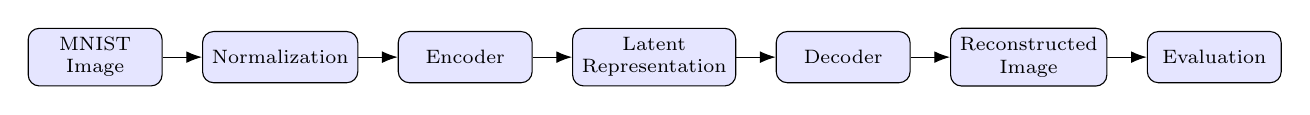
\begin{tikzpicture}[node distance=5mm]
\node[layer](a){MNIST\\Image};
\node[layer,right=of a](b){Normalization};
\node[layer,right=of b](c){Encoder};
\node[layer,right=of c](d){Latent\\Representation};
\node[layer,right=of d](e){Decoder};
\node[layer,right=of e](f){Reconstructed\\Image};
\node[layer,right=of f](g){Evaluation};

\foreach \x/\y in {a/b,b/c,c/d,d/e,e/f,f/g}
\draw[arrow](\x)--(\y);
\end{tikzpicture}
\end{center}

The experiment consists of four related studies:

\begin{enumerate}
\item Fully Connected Autoencoder
\item Convolutional Autoencoder
\item Denoising Convolutional Autoencoder
\item Variational Autoencoder
\end{enumerate}


%%%%%%%%%%%%%%%%%%%%%%%%%%%%%%%%%%%%%%%%%%%%%%%%%%%%%%%%%%%%
\section*{6. Exploring Autoencoders}

An autoencoder learns to reproduce its input at the output.

The encoder maps the input to a lower-dimensional representation:

\[
z=f_{\theta}(x),
\]

and the decoder reconstructs the input:

\[
\hat{x}=g_{\phi}(z).
\]

The training objective is to minimize reconstruction error:

\[
\mathcal{L}_{rec}
=
\frac{1}{N}\sum_{i=1}^{N}
\|x_i-\hat{x}_i\|^2.
\]

\begin{center}
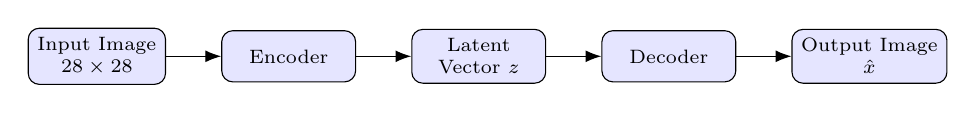
\begin{tikzpicture}[node distance=7mm]
\node[layer](a){Input Image\\$28\times28$};
\node[layer,right=of a](b){Encoder};
\node[layer,right=of b](c){Latent\\Vector $z$};
\node[layer,right=of c](d){Decoder};
\node[layer,right=of d](e){Output Image\\$\hat{x}$};

\foreach \x/\y in {a/b,b/c,c/d,d/e}
\draw[arrow](\x)--(\y);
\end{tikzpicture}
\end{center}

The latent vector is a compressed representation of the input.

\subsection*{Why the Bottleneck Matters, and Which Loss Was Used}

If the latent vector were as large as the input, the network could simply copy
its input and learn nothing useful. Making $z$ smaller than $x$ (an undercomplete
autoencoder) forces the encoder to keep what the decoder needs most, which is
the shape and layout of the stroke. For the FC model in Section 7 the
compression is $784\rightarrow16$, a factor of 49.

The autoencoders were trained with binary cross-entropy (BCE) instead of the
squared error written above. With pixels in $[0,1]$ and a sigmoid output, each
pixel can be read as a probability, and BCE punishes a confidently wrong pixel
more strongly than MSE. Evaluation, however, uses MSE, MAE and SSIM, which are
easier to interpret on the image scale, so the BCE values printed during
training should not be compared directly with the tables of results.

%%%%%%%%%%%%%%%%%%%%%%%%%%%%%%%%%%%%%%%%%%%%%%%%%%%%%%%%%%%%
\section*{7. Fully Connected Autoencoder}

Flatten each image from

\[
28\times28=784
\]

to a vector of length 784.

Use the following architecture:

\begin{center}
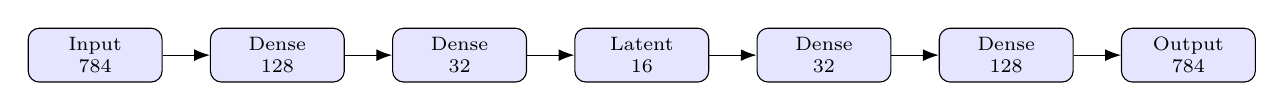
\begin{tikzpicture}[node distance=6mm]
\node[layer](a){Input\\784};
\node[layer,right=of a](b){Dense\\128};
\node[layer,right=of b](c){Dense\\32};
\node[layer,right=of c](d){Latent\\16};
\node[layer,right=of d](e){Dense\\32};
\node[layer,right=of e](f){Dense\\128};
\node[layer,right=of f](g){Output\\784};

\foreach \x/\y in {a/b,b/c,c/d,d/e,e/f,f/g}
\draw[arrow](\x)--(\y);
\end{tikzpicture}
\end{center}

Use ReLU activation in hidden layers and sigmoid activation in the output
layer.

\textbf{Suggested configuration:}

\begin{center}
\begin{tabular}{|l|l|}
\hline
Parameter & Value\\
\hline
Latent dimension & 16\\
Optimizer & Adam\\
Learning rate & $10^{-3}$\\
Batch size & 128\\
Epochs & 20\\
Loss & Binary Cross-Entropy\\
\hline
\end{tabular}
\end{center}

\subsection*{Layer-wise Parameter Count}

\begin{center}
\begin{tabular}{|l|c|c|}
\hline
Layer & Output shape & Parameters\\
\hline
Dense (ReLU) & 128 & 100,480\\
Dense (ReLU) & 32 & 4,128\\
Dense, latent (ReLU) & 16 & 528\\
Dense (ReLU) & 32 & 544\\
Dense (ReLU) & 128 & 4,224\\
Dense (sigmoid) & 784 & 101,136\\
\hline
\textbf{Total} & & \textbf{211,040}\\
\hline
\end{tabular}
\end{center}

Almost all of the parameters (about 96\%) sit in the first and the last layer,
which connect the 784 pixels to the 128-unit hidden layers. The latent layer
itself contributes only 528 parameters. The latent layer also uses ReLU, as
the manual asks for ReLU in the hidden layers, which means the 16 code values
are constrained to be non-negative.

\subsection*{Training Behaviour}

Each epoch has 79 steps (10,000 images at a batch size of 128). The training
BCE fell from 0.3468 in the first epoch to 0.1229 in the twentieth, and the
validation BCE fell from 0.2493 to 0.1228. Training took 16.14 s, of which
about 6 s belonged to the first epoch alone (graph construction and start-up).

%%%%%%%%%%%%%%%%%%%%%%%%%%%%%%%%%%%%%%%%%%%%%%%%%%%%%%%%%%%%
\section*{8. Required Analysis of the Basic Autoencoder}

\textbf{Plot 1: Original versus Reconstructed Images}

Display at least 10 test images in a grid.

For every image, show:

\[
\text{Original}\quad|\quad\text{Reconstruction}.
\]

Students must comment on:

\begin{itemize}
\item preservation of digit shape;
\item loss of fine details;
\item blurred regions;
\item differences between easy and difficult samples.
\end{itemize}

\textbf{Plot 2: Training and Validation Reconstruction Loss}

\begin{itemize}
\item X-axis: Epoch
\item Y-axis: Reconstruction loss
\item Curves: Training loss and validation loss
\end{itemize}

\textbf{Required inference:} Determine whether the model converges and whether
there is evidence of overfitting.

\begin{figure}[!htb]
\centering
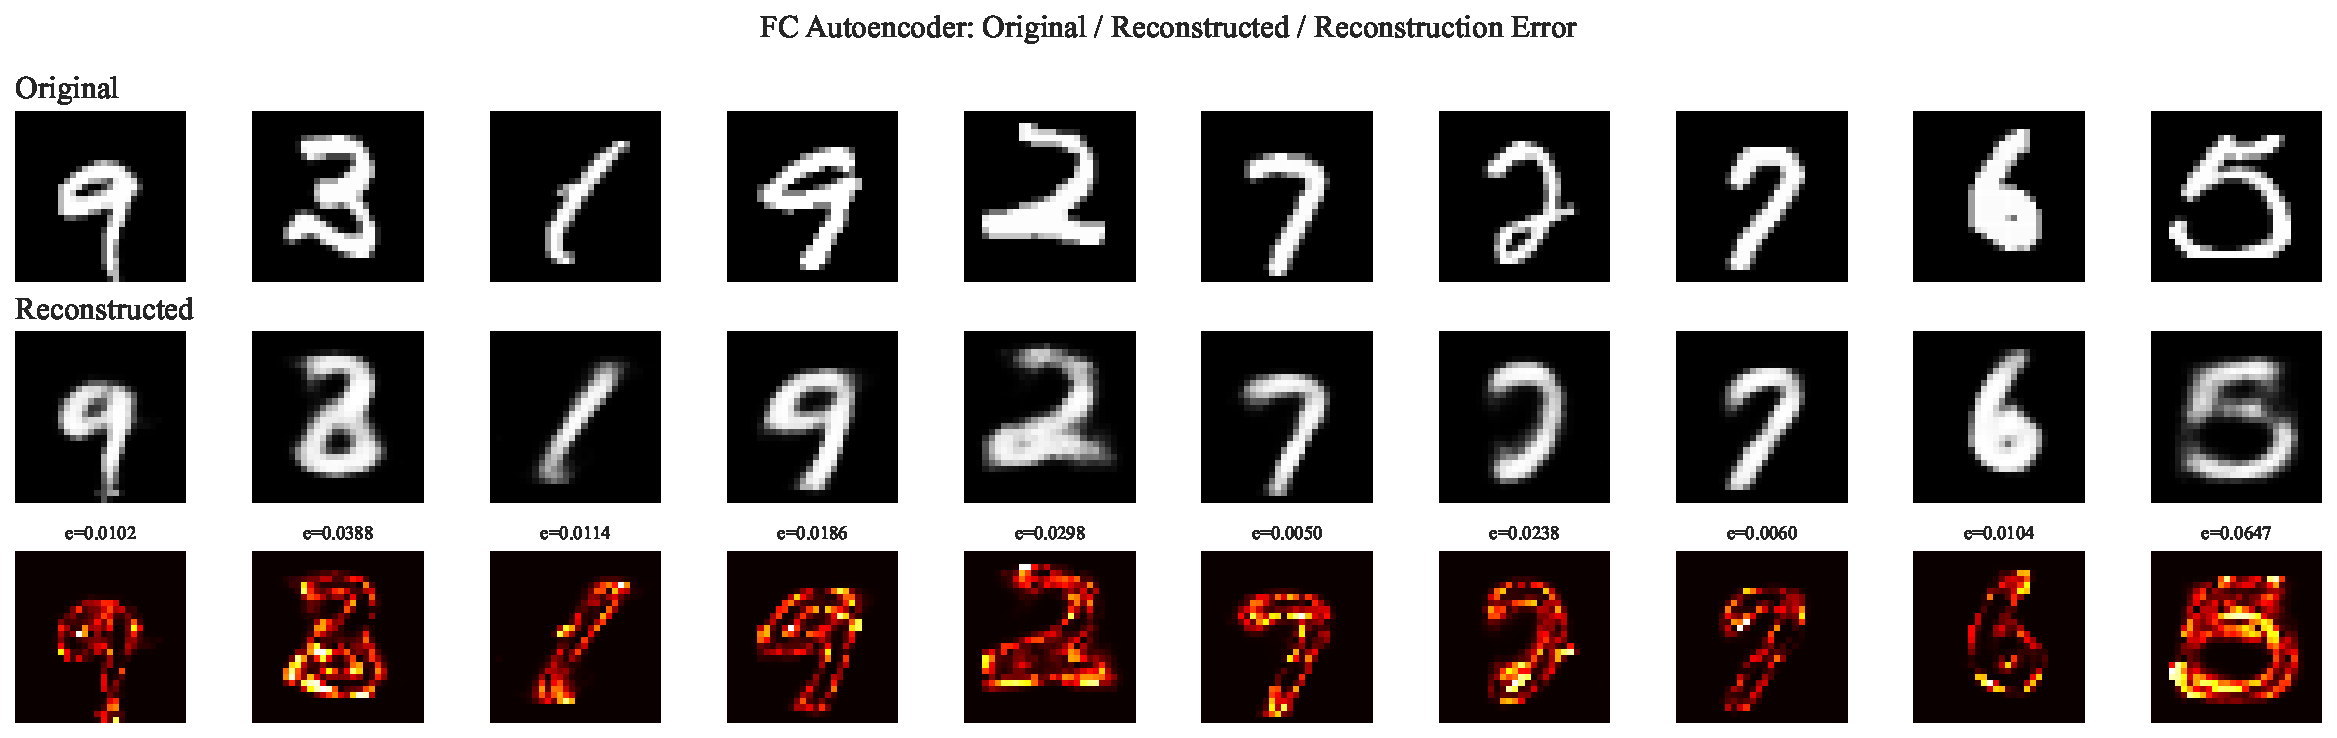
\includegraphics[width=0.86\linewidth]{Plot1_Original_vs_Reconstructed}
\caption{Plot 1: original test images (top), fully connected AE reconstructions (middle) and per-pixel absolute error with the per-image error $e$ (bottom).}
\label{fig:plot1}
\end{figure}

\subsection*{Observations on Plot 1}

The overall identity of most digits survives the $784\rightarrow16$ compression.
The 9, both 7s, the 6 and the 1 are recognisable, and the compact, thick-stroked
digits are reconstructed best (the 7s with $e=0.0050$ and $0.0060$, the 6 with
$e=0.0104$).

The error maps are bright almost only along stroke outlines and dark on the
background and inside thick strokes, which is what a blurring model produces:
stroke positions are roughly right but exact edges are not. Digits with loops,
corners and crossings (3, 5, 2) are harder than digits made of one simple stroke
(1, 7), because a 16-number code has to describe all those junctions together.

\begin{figure}[!htb]
\centering
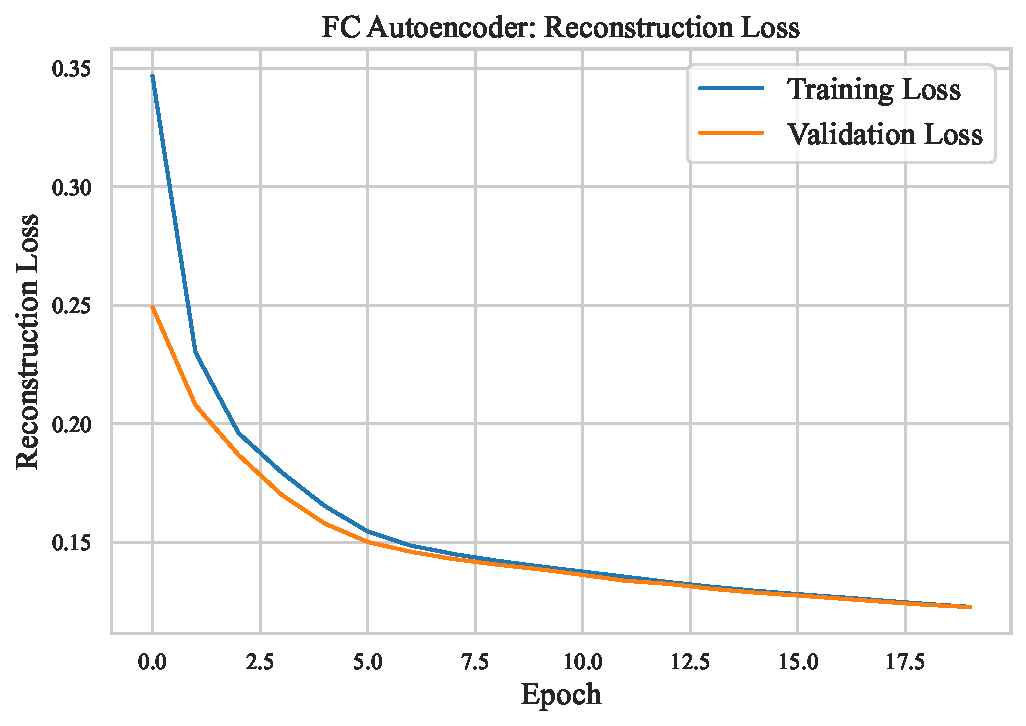
\includegraphics[width=0.6\linewidth]{Plot2_FC_Training_Validation_Loss}
\caption{Plot 2: training and validation reconstruction loss (BCE) of the fully connected autoencoder over 20 epochs.}
\label{fig:plot2}
\end{figure}

\subsection*{Inference from Plot 2}

\textbf{What the plot shows.} Both curves fall steeply in the first five epochs
(from about 0.35 and 0.25 to about 0.165 and 0.158) and then continue to
decrease slowly, ending at 0.1229 (training) and 0.1228 (validation).

\textbf{Trend and cause.} The validation loss stays slightly below the training
loss for almost the whole run and the two meet at epoch 20. Keras reports the training loss as an
average over the epoch, while the weights are still improving, whereas the
validation loss is computed once at the end of the epoch with the latest
weights. There is no dropout or other regularisation in this model that would
make training harder than validation.

\textbf{Conclusion.} The model converges without any sign of overfitting, since
the validation loss never turns upward. It has, however, not fully flattened
out by epoch 20: the training loss was still dropping by about 0.001 per epoch.

%%%%%%%%%%%%%%%%%%%%%%%%%%%%%%%%%%%%%%%%%%%%%%%%%%%%%%%%%%%%
\section*{9. Reconstruction Metrics}

Students must calculate the following metrics on the test set.

\subsection*{Mean Squared Error}

\[
MSE=
\frac{1}{N}
\sum_{i=1}^{N}
(x_i-\hat{x}_i)^2.
\]

\subsection*{Mean Absolute Error}

\[
MAE=
\frac{1}{N}
\sum_{i=1}^{N}
|x_i-\hat{x}_i|.
\]

\subsection*{Structural Similarity}

Calculate SSIM between the original and reconstructed images.

The implementation may use:

\url{https://scikit-image.org/docs/stable/api/skimage.metrics.html}

Report:

\begin{center}
\begin{tabular}{|l|c|}
\hline
Metric & Value\\
\hline
Test MSE & 0.019970\\
Test MAE & 0.054288\\
Mean SSIM & 0.7735\\
\hline
\end{tabular}
\end{center}

\subsection*{Reading the Numbers}

The MSE is averaged over all pixels and all test images, and SSIM was computed
image by image with the scikit-image default window and then averaged. An MSE of
0.0200 corresponds to a root-mean-square error of about 0.141 on the grey scale,
while the MAE is only 0.054. The RMSE is about 2.6 times the MAE, so the error is
concentrated in a small number of pixels (stroke edges, as in Plot 1) while the
dark background contributes almost nothing. SSIM is the stricter measure: blurring
a stroke changes local contrast and structure, so the mean SSIM is only 0.7735.
The metrics agree with the pictures, since the FC autoencoder gets the coarse
layout right but not the fine structure.

%%%%%%%%%%%%%%%%%%%%%%%%%%%%%%%%%%%%%%%%%%%%%%%%%%%%%%%%%%%%
\section*{10. Convolutional Autoencoder}

A Convolutional Autoencoder preserves spatial structure and uses convolutional
operations in the encoder and upsampling/transposed convolution operations
in the decoder.

The conceptual architecture is:

\begin{center}
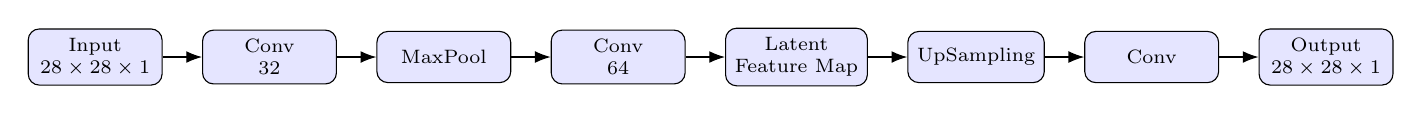
\begin{tikzpicture}[node distance=5mm]
\node[layer](a){Input\\$28\times28\times1$};
\node[layer,right=of a](b){Conv\\32};
\node[layer,right=of b](c){MaxPool};
\node[layer,right=of c](d){Conv\\64};
\node[layer,right=of d](e){Latent\\Feature Map};
\node[layer,right=of e](f){UpSampling};
\node[layer,right=of f](g){Conv};
\node[layer,right=of g](h){Output\\$28\times28\times1$};

\foreach \x/\y in {a/b,b/c,c/d,d/e,e/f,f/g,g/h}
\draw[arrow](\x)--(\y);
\end{tikzpicture}
\end{center}

A possible implementation is:

\begin{verbatim}
Input(28,28,1)
Conv2D(32, 3, activation='relu', padding='same')
MaxPooling2D(2, padding='same')
Conv2D(64, 3, activation='relu', padding='same')
MaxPooling2D(2, padding='same')
Conv2D(64, 3, activation='relu', padding='same')
UpSampling2D(2)
Conv2D(32, 3, activation='relu', padding='same')
UpSampling2D(2)
Conv2D(1, 3, activation='sigmoid', padding='same')
\end{verbatim}

The exact implementation may use Conv2DTranspose instead of UpSampling2D.

\subsection*{Layer-wise Shapes and Parameters}

\begin{center}
\begin{tabular}{|l|c|c|}
\hline
Layer & Output shape & Parameters\\
\hline
Conv2D(32, 3, ReLU) & $28\times28\times32$ & 320\\
MaxPooling2D(2) & $14\times14\times32$ & 0\\
Conv2D(64, 3, ReLU) & $14\times14\times64$ & 18,496\\
MaxPooling2D(2) & $7\times7\times64$ & 0\\
Conv2D(64, 3, ReLU) -- latent map & $7\times7\times64$ & 36,928\\
UpSampling2D(2) & $14\times14\times64$ & 0\\
Conv2D(32, 3, ReLU) & $14\times14\times32$ & 18,464\\
UpSampling2D(2) & $28\times28\times32$ & 0\\
Conv2D(1, 3, sigmoid) & $28\times28\times1$ & 289\\
\hline
\textbf{Total} & & \textbf{74,497}\\
\hline
\end{tabular}
\end{center}

\subsection*{Training Behaviour and a Remark on the Bottleneck}

Training BCE fell from 0.2480 to 0.0685 and validation BCE from 0.1039 to
0.0679 over 20 epochs (21.90 s in total). The validation loss was again
marginally below the training loss at the end and was still decreasing very
slowly, so the same remarks made for Plot 2 apply here.

The latent feature map of this architecture is $7\times7\times64=3136$ values, which
is more numbers than the 784 input pixels. It is therefore not a compression in
the same sense as the 16-dimensional code of the FC model, and this matters when
the two are compared in Section 11. The CAE was repeated with a real
low-dimensional bottleneck in Section 29.1.

%%%%%%%%%%%%%%%%%%%%%%%%%%%%%%%%%%%%%%%%%%%%%%%%%%%%%%%%%%%%
\section*{11. Comparing Fully Connected and Convolutional Autoencoders}

Train both models using the same training and test images.

\begin{center}
\begin{tabular}{|l|c|c|c|c|}
\hline
Model & MSE & MAE & SSIM & Parameters\\
\hline
Fully Connected AE & 0.019970 & 0.054288 & 0.7735 & 211,040\\
Convolutional AE & 0.002448 & 0.014828 & 0.9761 & 74,497\\
\hline
\end{tabular}
\end{center}

\textbf{Plot 3: Reconstruction Comparison}

Display:

\[
\text{Original}
\rightarrow
\text{FC-AE Reconstruction}
\rightarrow
\text{CAE Reconstruction}.
\]

\textbf{Required inference:}

Discuss how preserving spatial locality through convolution affects image
reconstruction.

\begin{figure}[!htb]
\centering
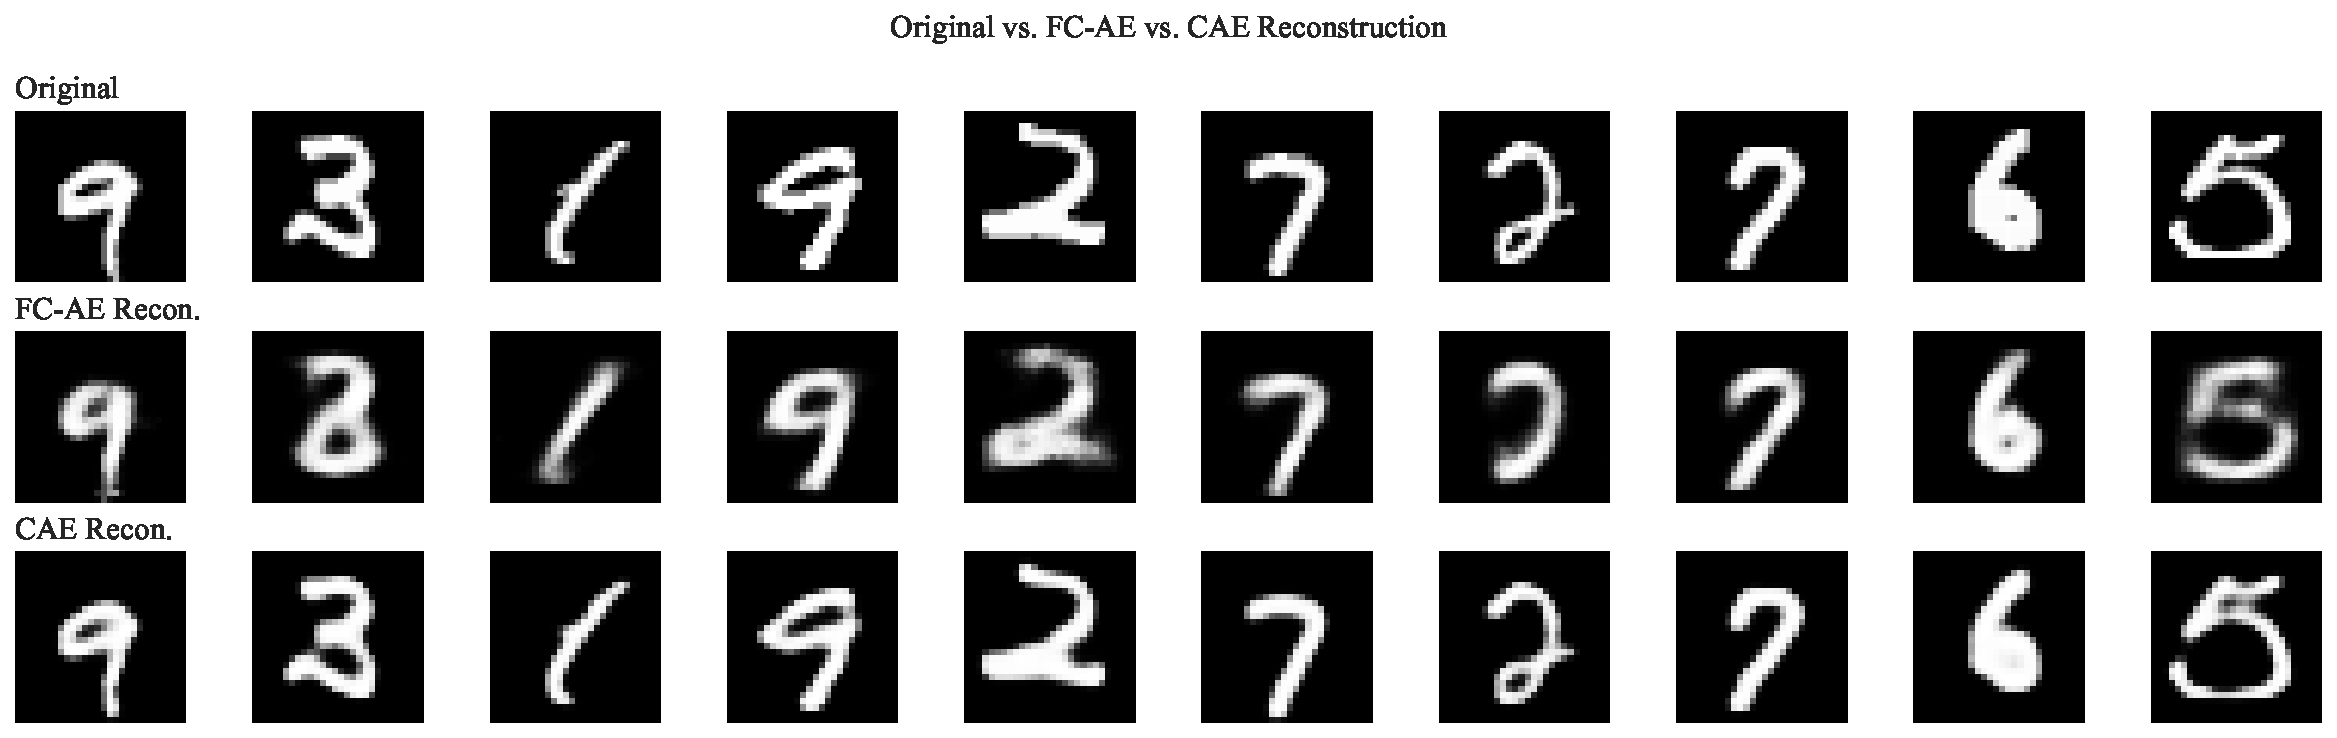
\includegraphics[width=0.86\linewidth]{Plot3_FC_vs_CAE_Reconstruction}
\caption{Plot 3: original test images (top), FC-AE reconstruction (middle) and convolutional AE reconstruction (bottom).}
\label{fig:plot3}
\end{figure}

\subsection*{Inference from Plot 3 and the Table}

\textbf{What the results show.} The convolutional autoencoder is better on every
metric. Its MSE is about 8.2 times lower (0.0024 against 0.0200), its MAE is
about 3.7 times lower, and its SSIM is 0.976 against 0.774. It also uses about
65\% fewer parameters (74,497 against 211,040).

\textbf{Why it happens.} A convolution looks at a small neighbourhood and
reuses the same filter at every position. A stroke edge looks the same wherever
it appears in the image, so a 3$\times$3 filter learned once is useful
everywhere, and this needs far fewer weights than a dense layer that has to
learn each pixel-to-unit connection separately.

\textbf{A fair-comparison caveat.} The two models do not have the same bottleneck:
the FC model squeezes the image into 16 numbers, while the CAE keeps a
$7\times7\times64$ map (3136 values), so part of the gap comes from the extra
room. With both models restricted to latent vector of the same size the CAE is still better, but the gap shrinks from eight-fold to
about two-fold in MSE.

%%%%%%%%%%%%%%%%%%%%%%%%%%%%%%%%%%%%%%%%%%%%%%%%%%%%%%%%%%%%
\section*{12. Denoising Autoencoder}

A denoising autoencoder receives a corrupted image but is trained to
reconstruct the original clean image.

The training mapping is:

\[
\boxed{\tilde{x}\rightarrow\text{Encoder}\rightarrow z
\rightarrow\text{Decoder}\rightarrow\hat{x}}
\]

where $\tilde{x}$ is a noisy version of the clean image $x$.

\begin{center}
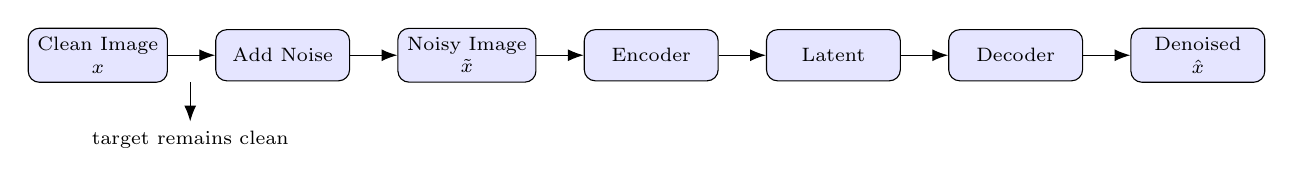
\begin{tikzpicture}[node distance=6mm]
\node[layer](a){Clean Image\\$x$};
\node[layer,right=of a](b){Add Noise};
\node[layer,right=of b](c){Noisy Image\\$\tilde{x}$};
\node[layer,right=of c](d){Encoder};
\node[layer,right=of d](e){Latent};
\node[layer,right=of e](f){Decoder};
\node[layer,right=of f](g){Denoised\\$\hat{x}$};

\foreach \x/\y in {a/b,b/c,c/d,d/e,e/f,f/g}
\draw[arrow](\x)--(\y);

\draw[arrow]($(a.south)!0.5!(b.south)$) -- ++(0,-5mm)
node[below,font=\scriptsize]{target remains clean};
\end{tikzpicture}
\end{center}

\subsection*{Why Not Simply Copy the Input?}

If the network were trained to map $\tilde{x}\rightarrow\tilde{x}$, the best solution
would be the identity, noise included. With the clean image as the target, the
only way to lower the loss is to learn what digits look like and drop whatever
does not fit. The noise is random and repeats no pattern from image to image, so
the network cannot predict it and learns to ignore it.

The model used here has the same architecture as the CAE in Section 10, with
the same 74,497 parameters. The only change is in the data: it was trained on
inputs corrupted with Gaussian noise of $\sigma=0.2$, with the clean image as
the target. The training BCE fell from 0.2496 to 0.0758 and the validation BCE
from 0.1218 to 0.0753 (20.00 s). Compared with the clean CAE (0.0685 and 0.0679)
the final loss is higher by about 0.007. That gap is the price of having to
undo the noise.

%%%%%%%%%%%%%%%%%%%%%%%%%%%%%%%%%%%%%%%%%%%%%%%%%%%%%%%%%%%%
\section*{13. Adding Image Noise}

Use at least two corruption types.

\subsection*{Gaussian Noise}

\[
\tilde{x}=x+n,
\qquad
n\sim\mathcal{N}(0,\sigma^2).
\]

Suggested standard deviations:

\[
\sigma\in\{0.1,0.2,0.3\}.
\]

Clip the resulting image to the range $[0,1]$.

\subsection*{Salt-and-Pepper Noise}

Randomly replace a small proportion of pixels with values close to 0 or 1.

Suggested corruption levels:

\[
p\in\{0.05,0.10,0.20\}.
\]

\subsection*{Implementation Details}

Gaussian noise was added with a seeded NumPy generator and the result was clipped
to $[0,1]$. For salt-and-pepper noise a uniform random number was drawn for every
pixel: values below $p/2$ were set to 0 (pepper), values between $p/2$ and $p$ were
set to 1 (salt), and the rest were left untouched, so a fraction $p$ of the pixels
is corrupted. Both noisy versions were checked to stay within 0 and 1.

Different seeds were used for the training noise and the test noise (42 and 43),
so the network never meets the same noise pattern at test time that it saw in
training.

%%%%%%%%%%%%%%%%%%%%%%%%%%%%%%%%%%%%%%%%%%%%%%%%%%%%%%%%%%%%
\section*{14. Required Denoising Plots}

\textbf{Plot 4: Clean vs. Noisy vs. Denoised}

For at least 10 images, display:

\[
\text{Clean}\quad|\quad
\text{Noisy}\quad|\quad
\text{Denoised}.
\]

\textbf{Plot 5: Noise Level vs. Reconstruction Quality}

For each noise level, calculate:

\[
MSE,\quad MAE,\quad SSIM.
\]

Report:

\begin{center}
\begin{tabular}{|c|c|c|c|}
\hline
Noise Level & MSE & MAE & SSIM\\
\hline
0.1 & 0.003593 & 0.017905 & 0.9616\\
0.2 & 0.004533 & 0.021190 & 0.9478\\
0.3 & 0.006963 & 0.029143 & 0.8819\\
\hline
\end{tabular}
\end{center}

\textbf{Required inference:}

Explain how increasing corruption affects reconstruction quality and identify
whether the denoising model is able to recover the major structure of the
original image.

\begin{figure}[!htb]
\centering
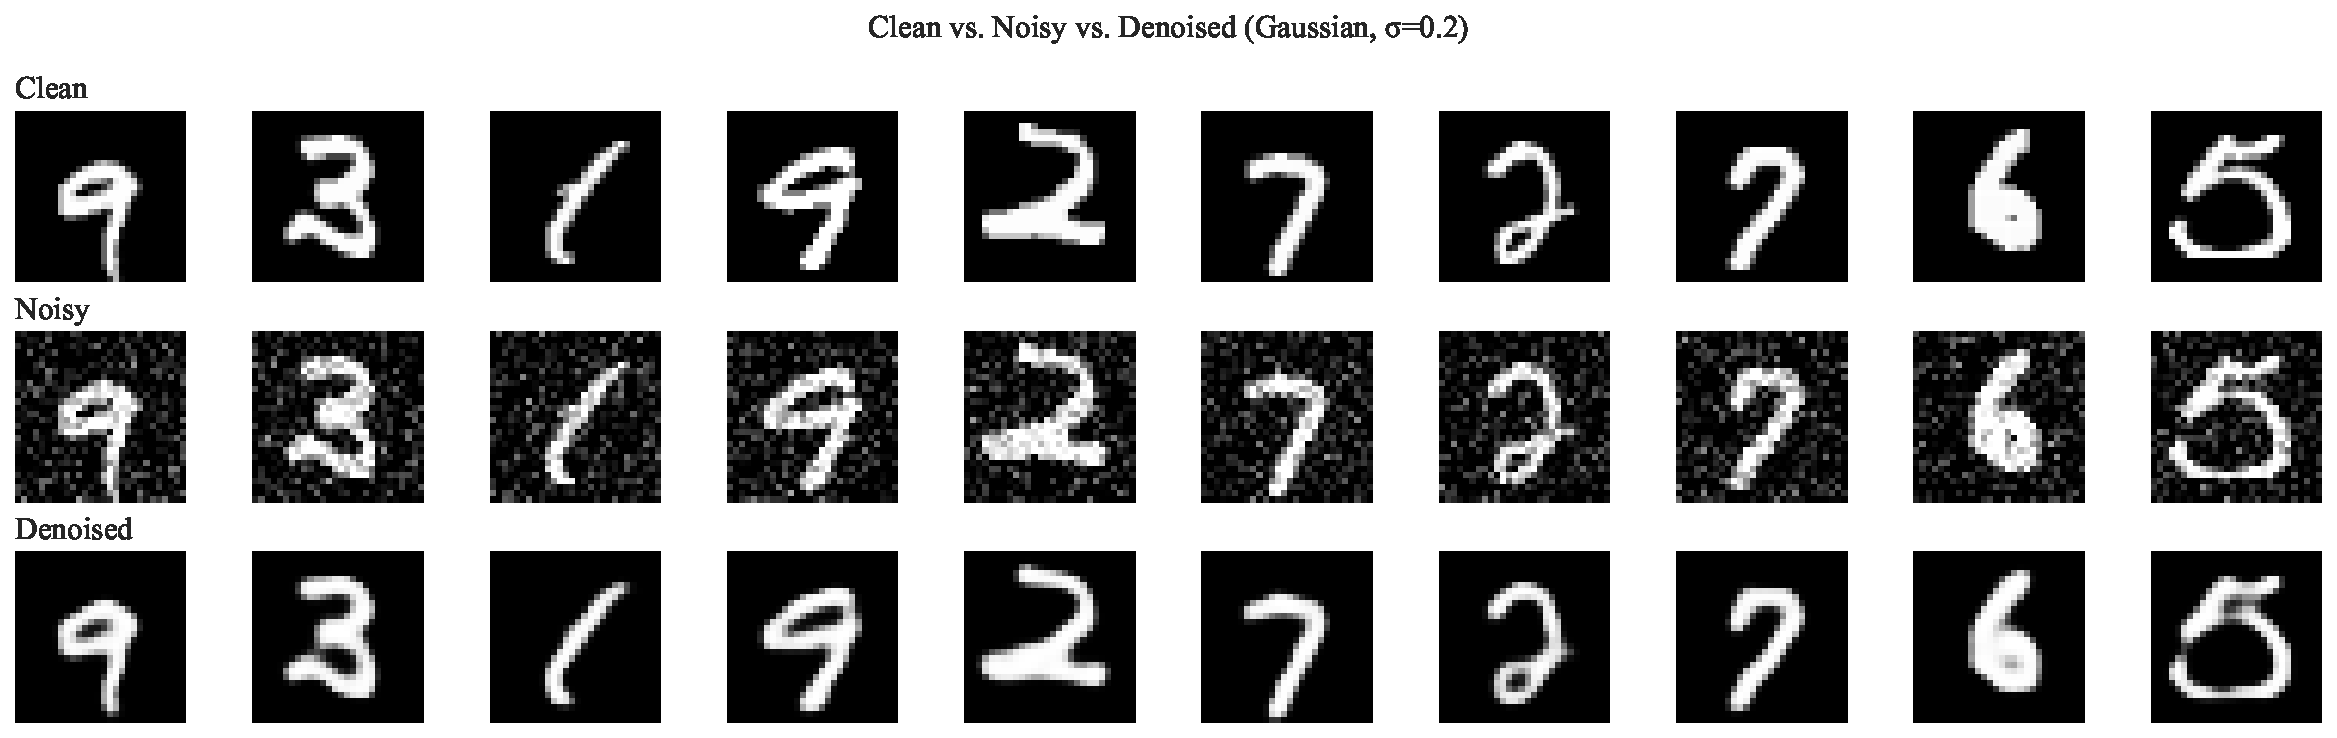
\includegraphics[width=0.86\linewidth]{Plot4_Clean_Noisy_Denoised}
\caption{Plot 4: clean test images (top), the same images with Gaussian noise of $\sigma=0.2$ (middle) and the output of the denoising CAE (bottom).}
\label{fig:plot4}
\end{figure}

\subsection*{Observations on Plot 4}

The noisy row is clearly degraded: the background is speckled and thin strokes,
some are partly broken up. In the denoised row the
background is clean again and the strokes are continuous. Strokes again become somewhat
little thicker and softer than in the clean originals, and very fine details are smoothed. Even
so, all ten digits remain correctly identifiable.

\begin{figure}[!htb]
\centering
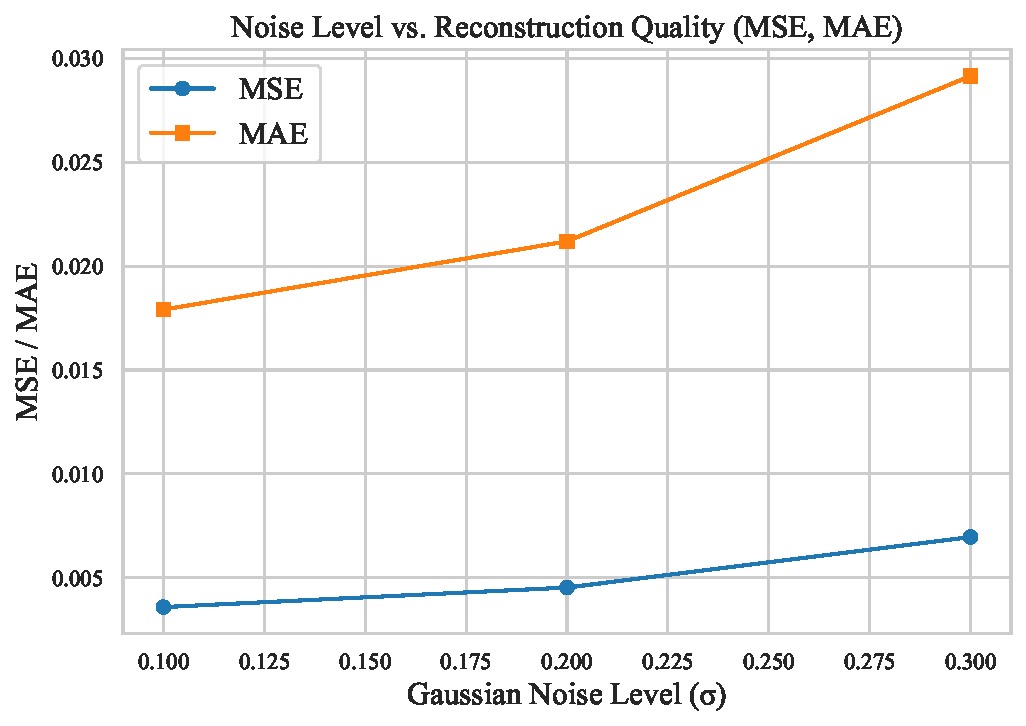
\includegraphics[width=0.5\linewidth]{Plot5a_NoiseLevel_vs_MSE_MAE}\hspace{4mm}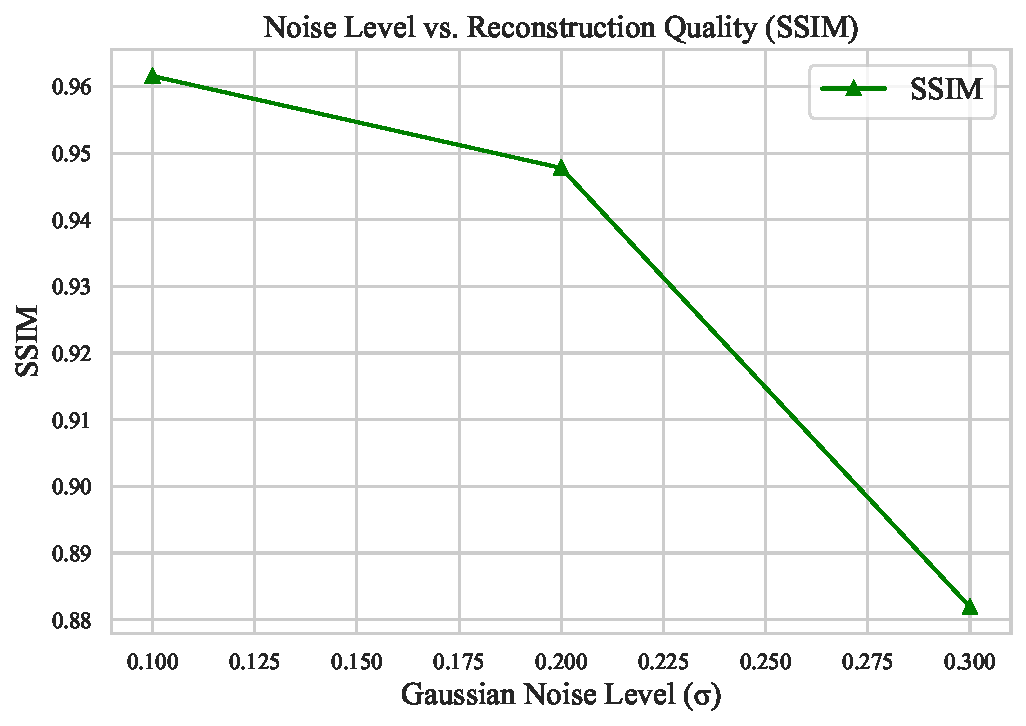
\includegraphics[width=0.5\linewidth]{Plot5b_NoiseLevel_vs_SSIM}
\caption{Plot 5: effect of the Gaussian noise level $\sigma$ on the denoiser. Left: MSE and MAE. Right: mean SSIM.}
\label{fig:plot5}
\end{figure}

\subsection*{Inference from Plot 5}

\textbf{What the plots show.} All three measures degrade as the noise grows. The
change is not linear. From $\sigma=0.1$ to 0.2 the MSE rises by 26\% and SSIM
falls by 0.014, while from 0.2 to 0.3 the MSE rises by 54\% and SSIM falls by
0.066.

\textbf{Conclusion.} The denoiser recovers the major structure at every tested
level. Even at $\sigma=0.3$ the output is a readable digit and not a blank or
noisy image, so the model has learned what digits look like and not a pixel-wise
copy. What is lost is fine detail, and the loss grows quickly once the noise is
comparable with the stroke intensity.

%%%%%%%%%%%%%%%%%%%%%%%%%%%%%%%%%%%%%%%%%%%%%%%%%%%%%%%%%%%%
\section*{15. Variational Autoencoder}

A conventional autoencoder maps an input to a deterministic latent vector:

\[
z=f(x).
\]

A VAE instead learns a probability distribution:

\[
q_{\phi}(z|x)
=
\mathcal{N}
\left(
\mu(x),
\operatorname{diag}(\sigma^2(x))
\right).
\]

The encoder produces:

\[
\mu,\qquad \log\sigma^2.
\]

A latent vector is sampled using the reparameterization trick:

\[
z=\mu+\sigma\odot\epsilon,
\qquad
\epsilon\sim\mathcal{N}(0,I).
\]

\begin{center}
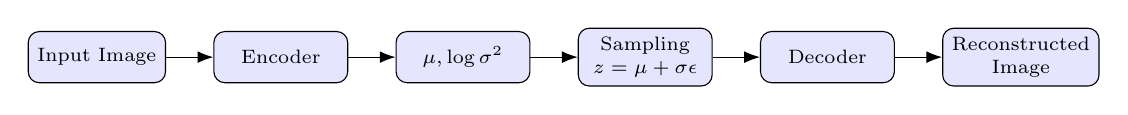
\begin{tikzpicture}[node distance=6mm]
\node[layer](a){Input Image};
\node[layer,right=of a](b){Encoder};
\node[layer,right=of b](c){$\mu,\log\sigma^2$};
\node[layer,right=of c](d){Sampling\\$z=\mu+\sigma\epsilon$};
\node[layer,right=of d](e){Decoder};
\node[layer,right=of e](f){Reconstructed\\Image};

\foreach \x/\y in {a/b,b/c,c/d,d/e,e/f}
\draw[arrow](\x)--(\y);
\end{tikzpicture}
\end{center}

\subsection*{Two Practical Points}

The encoder outputs $\log\sigma^2$ instead of $\sigma$ so that the network
output can be any real number while the variance $\sigma^2=e^{\log\sigma^2}$ is
always positive, and training is numerically better behaved. In the code the
sample is computed as $z=\mu+e^{0.5\log\sigma^2}\epsilon$.

The reparameterization trick moves the randomness into $\epsilon$, which does not
depend on any network weight, so $z$ is a differentiable function of $\mu$ and
$\sigma$ and gradients can flow from the decoder back into the encoder. Sampling
$z$ directly from $\mathcal{N}(\mu,\sigma^2)$ would block back-propagation at
that step.

%%%%%%%%%%%%%%%%%%%%%%%%%%%%%%%%%%%%%%%%%%%%%%%%%%%%%%%%%%%%
\section*{16. VAE Loss Function}

The VAE objective consists of two components.

\subsection*{Reconstruction Loss}

\[
\mathcal{L}_{rec}
=
-\mathbb{E}_{q_{\phi}(z|x)}
[\log p_{\theta}(x|z)].
\]

For normalized MNIST images, binary cross-entropy can be used.

\subsection*{KL Divergence}

\[
D_{KL}
\left(
q_{\phi}(z|x)\parallel p(z)
\right)
=
-\frac{1}{2}
\sum_j
\left(
1+\log\sigma_j^2-\mu_j^2-\sigma_j^2
\right).
\]

The total loss is

\[
\boxed{
\mathcal{L}_{VAE}
=
\mathcal{L}_{rec}
+
\mathcal{L}_{KL}
}
\]

where the prior is usually

\[
p(z)=\mathcal{N}(0,I).
\]

\subsection*{Scale of the Loss Values}

In the implementation the BCE was summed over the 784 pixels of each image
and then averaged over the batch, and the KL term was summed over the latent
dimensions. That is why the VAE losses are in the range of 170--190, while the
autoencoder losses above are about 0.1 (a per-pixel mean). Dividing the VAE
reconstruction loss of 172.9 by 784 gives about 0.22 per pixel, which is the
number that can be compared with the 0.12 per pixel of the FC autoencoder. The
KL term reported in the tables is the unweighted value, and the total loss used
for training is $\mathcal{L}_{rec}+w\,\mathcal{L}_{KL}$ with $w=1$ unless stated
otherwise (Section 29.6).

%%%%%%%%%%%%%%%%%%%%%%%%%%%%%%%%%%%%%%%%%%%%%%%%%%%%%%%%%%%%
\section*{17. VAE Implementation}

Use a small latent space so that it can be visualized.

Suggested latent dimension:

\[
z\in\mathbb{R}^{2}.
\]

The encoder should produce:

\[
\mu\in\mathbb{R}^{2},
\qquad
\log\sigma^2\in\mathbb{R}^{2}.
\]

The decoder maps

\[
z\rightarrow28\times28\times1.
\]

A compact architecture is:

\begin{center}
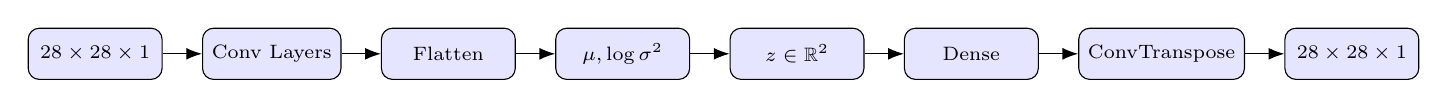
\begin{tikzpicture}[node distance=5mm]
\node[layer](a){$28\times28\times1$};
\node[layer,right=of a](b){Conv Layers};
\node[layer,right=of b](c){Flatten};
\node[layer,right=of c](d){$\mu,\log\sigma^2$};
\node[layer,right=of d](e){$z\in\mathbb{R}^2$};
\node[layer,right=of e](f){Dense};
\node[layer,right=of f](g){ConvTranspose};
\node[layer,right=of g](h){$28\times28\times1$};

\foreach \x/\y in {a/b,b/c,c/d,d/e,e/f,f/g,g/h}
\draw[arrow](\x)--(\y);
\end{tikzpicture}
\end{center}

\subsection*{Architecture Used}

\begin{center}
\begin{tabular}{|l|l|c|}
\hline
Part & Layer & Parameters\\
\hline
Encoder & Conv2D(32, 3, stride 2, ReLU) $\rightarrow14\times14\times32$ & 320\\
Encoder & Conv2D(64, 3, stride 2, ReLU) $\rightarrow7\times7\times64$ & 18,496\\
Encoder & Flatten $\rightarrow3136$, Dense(16, ReLU) & 50,192\\
Encoder & Dense(2) for $\mu$, Dense(2) for $\log\sigma^2$ & 68\\
Encoder & Sampling layer (reparameterization) & 0\\
\hline
Decoder & Dense($7\cdot7\cdot64$, ReLU), reshape & 9,408\\
Decoder & Conv2DTranspose(64, 3, stride 2, ReLU) & 36,928\\
Decoder & Conv2DTranspose(32, 3, stride 2, ReLU) & 18,464\\
Decoder & Conv2DTranspose(1, 3, sigmoid) $\rightarrow28\times28\times1$ & 289\\
\hline
\textbf{Total} & encoder 69,076 $+$ decoder 65,089 & \textbf{134,165}\\
\hline
\end{tabular}
\end{center}

A 16-unit dense layer sits between the convolutional stack and the two latent
heads, so all the information about the image passes through 16 numbers before
being reduced to the 2D code. This is a narrow path and probably limits the model.

\begin{figure}[!htb]
\centering
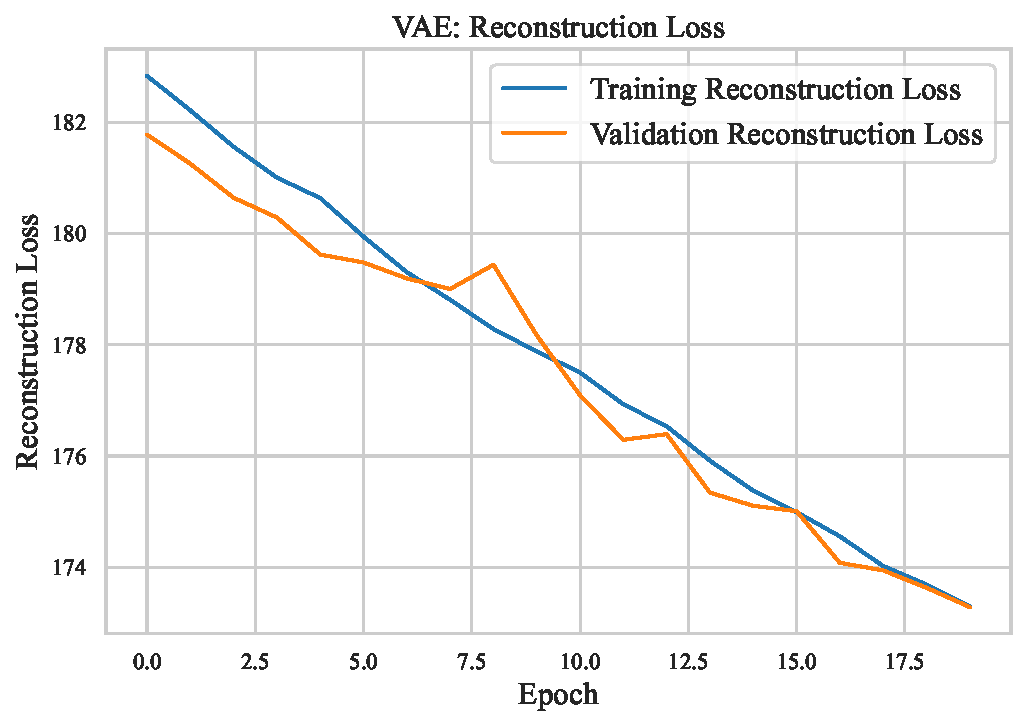
\includegraphics[width=0.5\linewidth]{PlotVAE_Training_Validation_Loss}
\caption{VAE reconstruction loss (summed BCE per image) on the training and validation images over 20 epochs.}
\label{fig:vaeloss}
\end{figure}

\subsection*{Inference from the VAE Training Curves}

The training reconstruction loss fell from 182.8 to 173.3 and the validation one
from 181.8 to 173.3, while the KL term rose slowly from 2.89 to 3.41 (validation
3.44). The two curves lie almost on top of each other, so there is no
overfitting, and the small bump in the validation loss at epoch 9 (182.19 to
182.77) is expected because a new random $\epsilon$ is drawn at each evaluation.
The loss is still decreasing at epoch 20, so the VAE has not converged, and the
20-epoch budget shared by all models is short for a VAE. The generation results
below should be read with that in mind.

%%%%%%%%%%%%%%%%%%%%%%%%%%%%%%%%%%%%%%%%%%%%%%%%%%%%%%%%%%%%
\section*{18. Exploring the VAE Latent Space}

Since the latent dimension is two, students can visualize the encoded test
images in a two-dimensional plane.

\textbf{Plot 6: VAE Latent Space}

\begin{itemize}
\item X-axis: $z_1$
\item Y-axis: $z_2$
\item Color/marker category: digit label
\end{itemize}

The labels are used only for visualization; they are not supplied to the VAE
during training.

\textbf{Required inference:}

Students should describe whether samples belonging to the same digit occupy
similar regions and whether different digits overlap.

\begin{figure}[!htb]
\centering
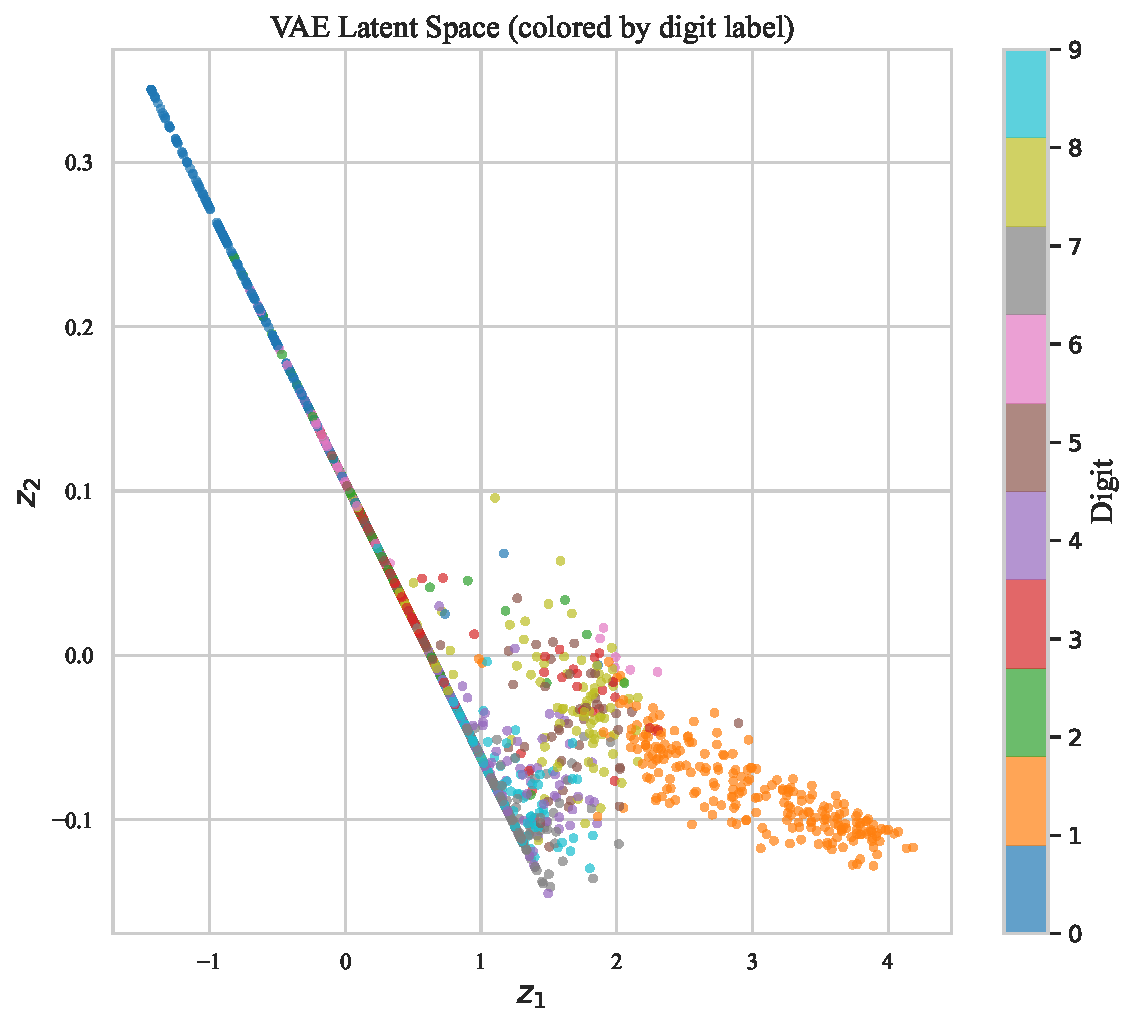
\includegraphics[width=0.46\linewidth]{Plot6_VAE_Latent_Space}
\caption{Plot 6: posterior means $(\mu_1,\mu_2)$ of the 2,000 test images, coloured by digit label (labels were not used in training).}
\label{fig:plot6}
\end{figure}

\subsection*{Inference from Plot 6}

\textbf{What the plot shows.} The encoded points do not fill the plane. They lie
almost along one thin line from the upper left to the lower right.

\textbf{Why, and conclusion.} A two-dimensional code can hold only a couple of
coarse image properties. The 0 (a big loop) and the 1 (a thin bar) differ most in
ink, so they are the easiest to put at opposite ends of the main axis, while the
other digits share similar strokes and cannot be separated by two numbers. The VAE has organised its space by overall shape
without seeing labels, but the space is largely collapsed onto one direction,
which explains the poor reconstruction and generation results that follow.

%%%%%%%%%%%%%%%%%%%%%%%%%%%%%%%%%%%%%%%%%%%%%%%%%%%%%%%%%%%%
\section*{19. Generating New Images with the VAE}

Sample points from

\[
z\sim\mathcal{N}(0,I).
\]

Pass the sampled latent vectors through the decoder.

\textbf{Plot 7: Randomly Generated Images}

Generate at least 25 images using randomly sampled latent vectors.

Display them in a grid.

Students should determine:

\begin{itemize}
\item whether the generated images resemble handwritten digits;
\item whether digit shapes are recognizable;
\item whether there is visible variation among generated samples; and
\item whether some samples are ambiguous or unrealistic.
\end{itemize}

\begin{figure}[!htb]
\centering
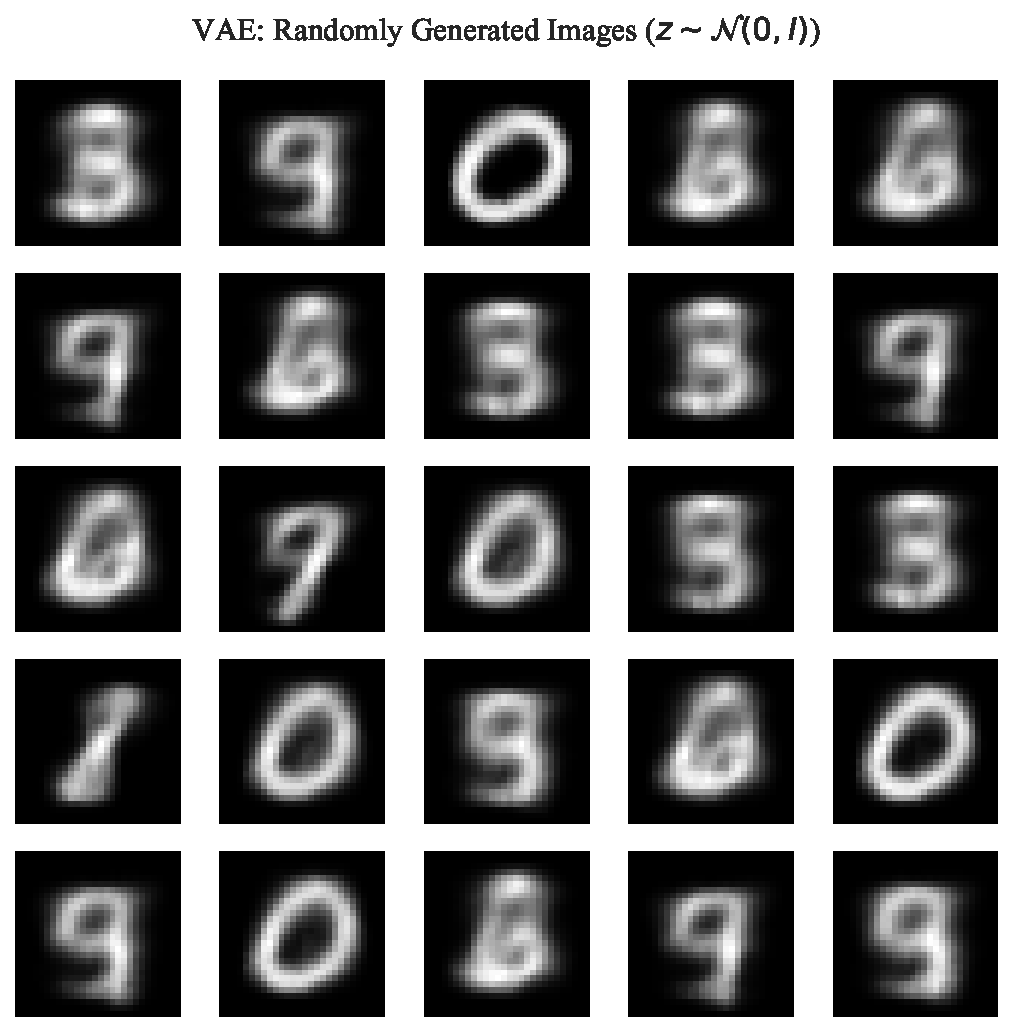
\includegraphics[width=0.42\linewidth]{Plot7_VAE_Random_Generated_Images}
\caption{Plot 7: 25 images generated by decoding random points $z\sim\mathcal{N}(0,I)$.}
\label{fig:plot7}
\end{figure}

\subsection*{Inference from Plot 7}

\textbf{Variation and quality.} Slant, thickness and width vary, but the variety
of classes is small: 2, 4 and 7 do not appear clearly and the same few shapes
repeat. Many samples are ambiguous, and the 5/3/8-like ones are blurred blobs with
grey interiors and much softer strokes than real handwriting.

\textbf{Why.} This follows from Plot 6. A random $z$ from $\mathcal{N}(0,I)$ mostly
lands in the crowded middle region where classes are mixed, and the decoder returns
an average of the overlapping digits, which looks like a blurred blend. Blurry
output is also typical of VAEs with a per-pixel likelihood, and the short training
and tiny latent space make it worse. The decoder has still learned something
meaningful (digit-like strokes and not noise), but the quality is modest.

%%%%%%%%%%%%%%%%%%%%%%%%%%%%%%%%%%%%%%%%%%%%%%%%%%%%%%%%%%%%
\section*{20. Latent Space Interpolation}

Select two latent vectors:

\[
z_A,\qquad z_B.
\]

Construct

\[
z(\alpha)=(1-\alpha)z_A+\alpha z_B,
\qquad
\alpha\in[0,1].
\]

Use values such as:

\[
\alpha=
0,\;0.1,\;0.2,\ldots,1.
\]

Decode every interpolated vector.

\textbf{Plot 8: Latent Space Interpolation}

Display the decoded images in sequence.

\textbf{Required inference:}

Describe whether the decoded image changes smoothly as the latent vector moves
between two points.

\begin{figure}[!htb]
\centering
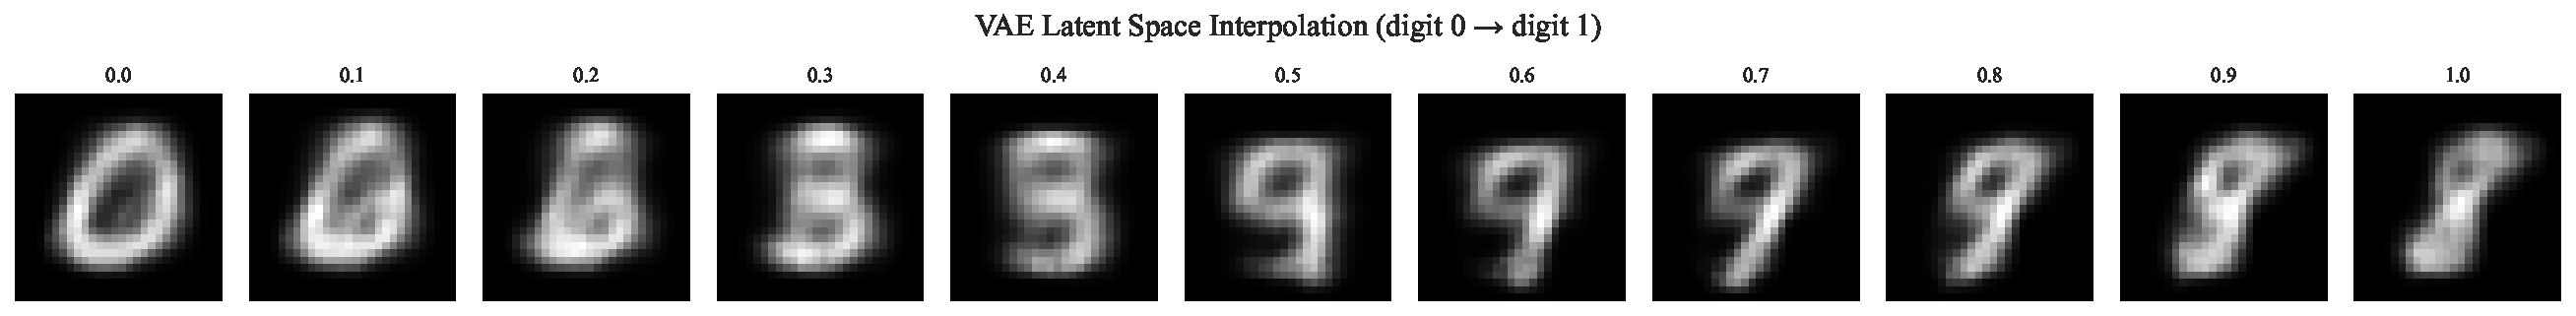
\includegraphics[width=0.86\linewidth]{Plot8_VAE_Latent_Interpolation}
\caption{Plot 8: decoded images along the straight line between the latent means of a test 0 ($\alpha=0$) and a test 1 ($\alpha=1$).}
\label{fig:plot8}
\end{figure}

\subsection*{Inference from Plot 8}

\textbf{What the plot shows.} The image changes gradually from frame to frame
with no sudden jump, which is the main property the VAE is meant to provide: small
steps in $z$ give small changes in the image.

\textbf{Conclusion.} The latent space is continuous but not semantically clean:
the transition from 0 to 1 is not a gradual thinning of a loop but goes through
other digit shapes.

%%%%%%%%%%%%%%%%%%%%%%%%%%%%%%%%%%%%%%%%%%%%%%%%%%%%%%%%%%%%
\section*{21. Reconstruction Comparison Across Models}

Compare the three reconstruction-based models:

\begin{center}
\begin{tabular}{|l|c|c|c|c|}
\hline
Model & MSE & MAE & SSIM & Parameters\\
\hline
Fully Connected AE & 0.019970 & 0.054288 & 0.7735 & 211,040\\
Convolutional AE & 0.002448 & 0.014828 & 0.9761 & 74,497\\
Denoising CAE & 0.004572 & 0.021277 & 0.9475 & 74,497\\
\hline
\end{tabular}
\end{center}

For the VAE, report its reconstruction loss separately because its total
objective also contains the KL-divergence term.

\begin{center}
\begin{tabular}{|l|c|}
\hline
VAE Metric & Value\\
\hline
Reconstruction Loss & 172.9133\\
KL Loss & 3.4480\\
Total Loss & 176.3613\\
Test MSE & 0.053703\\
Test MAE & 0.120811\\
Mean SSIM & 0.3791\\
\hline
\end{tabular}
\end{center}

\subsection*{Discussion}

The Denoising CAE row is measured against the clean image, but its input was the
noisy image ($\sigma=0.2$). It is therefore a harder task than the plain CAE,
and the loss of quality
is modest. The denoiser, which never sees a clean input, is still about 4.4
times better in MSE than the fully connected autoencoder, which does. The
architecture matters more than the noise here.

The VAE has by far the worst reconstruction numbers (MSE 0.0537, SSIM 0.379).
Four things in the set-up probably act together: the code has only two dimensions; the reconstruction is made from a \emph{sampled} $z$, so the
metrics also include sampling randomness that the deterministic models do not
have; the KL term pulls the codes towards $\mathcal{N}(0,I)$ and limits the
information they carry (KL is only 3.45 nats); and the VAE was still improving at
epoch 20 (Section 17).

%%%%%%%%%%%%%%%%%%%%%%%%%%%%%%%%%%%%%%%%%%%%%%%%%%%%%%%%%%%%
\section*{22. Required Plots}

The final report must contain the following plots:

\begin{enumerate}
\item Original image versus reconstructed image.
\item Training and validation loss for the basic autoencoder.
\item Fully connected AE versus convolutional AE reconstruction.
\item Clean versus noisy versus denoised images.
\item Noise level versus MSE/MAE/SSIM.
\item VAE latent-space visualization.
\item Randomly generated VAE images.
\item Latent-space interpolation.
\item Training/validation reconstruction loss for the VAE.
\item Reconstruction-error distribution on the test set.
\end{enumerate}

For plots containing multiple quantitative measures, use separate figures or
clearly labeled axes rather than placing incompatible scales on one axis.

\subsection*{Where Each Required Plot Appears}

\begin{center}
\begin{tabular}{|c|l|c|}
\hline
No. & Required plot & Figure\\
\hline
1 & Original versus reconstructed image & Fig.~\ref{fig:plot1}\\
2 & Training and validation loss, basic AE & Fig.~\ref{fig:plot2}\\
3 & FC-AE versus CAE reconstruction & Fig.~\ref{fig:plot3}\\
4 & Clean versus noisy versus denoised & Fig.~\ref{fig:plot4}\\
5 & Noise level versus MSE/MAE and SSIM & Fig.~\ref{fig:plot5}\\
6 & VAE latent-space visualization & Fig.~\ref{fig:plot6}\\
7 & Randomly generated VAE images & Fig.~\ref{fig:plot7}\\
8 & Latent-space interpolation & Fig.~\ref{fig:plot8}\\
9 & Training/validation loss for the VAE & Fig.~\ref{fig:vaeloss}\\
10 & Reconstruction-error distribution & Fig.~\ref{fig:plot9}\\
\hline
\end{tabular}
\end{center}


%%%%%%%%%%%%%%%%%%%%%%%%%%%%%%%%%%%%%%%%%%%%%%%%%%%%%%%%%%%%
\section*{23. Reconstruction Error Distribution}

Calculate the per-image reconstruction error:

\[
e_i=
\frac{1}{D}
\sum_{j=1}^{D}
(x_{ij}-\hat{x}_{ij})^2.
\]

\textbf{Plot 9: Distribution of Reconstruction Errors}

Plot a histogram of $e_i$ over the test set.

Students should identify:

\begin{itemize}
\item the typical reconstruction-error range;
\item whether the distribution is concentrated or spread out;
\item possible high-error samples; and
\item representative images corresponding to high reconstruction error.
\end{itemize}

\begin{figure}[!htb]
\centering
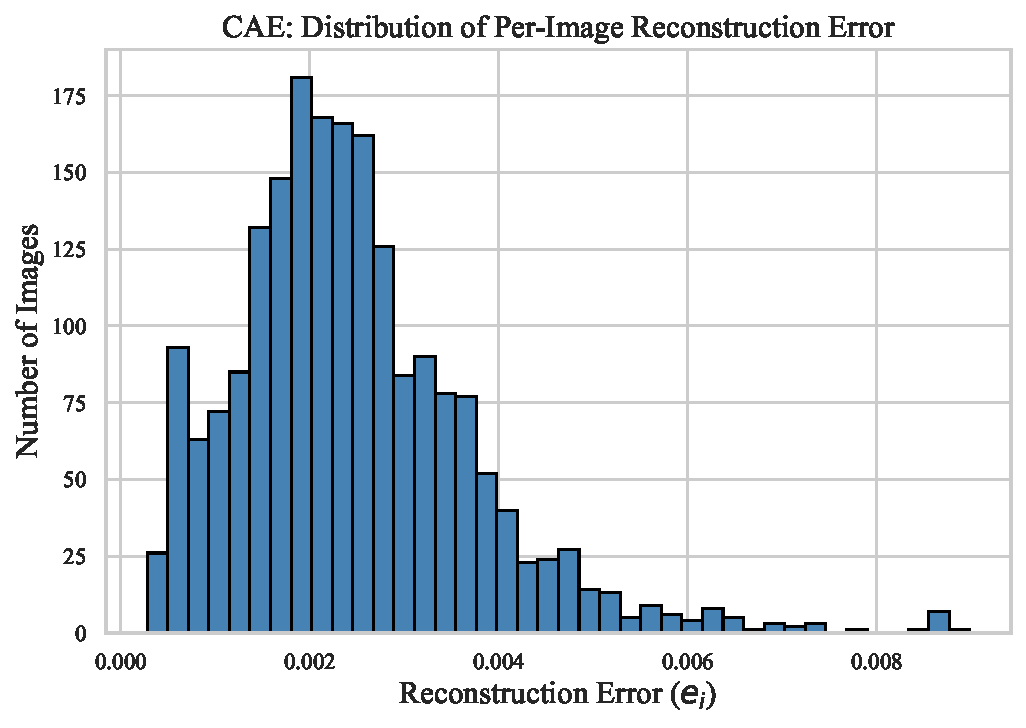
\includegraphics[width=0.42\linewidth]{Plot9_Reconstruction_Error_Distribution}
\caption{Plot 9: histogram of the per-image reconstruction error $e_i$ of the convolutional autoencoder on the 2,000 test images.}
\label{fig:plot9}
\end{figure}

\subsection*{Inference from Plot 9}

\textbf{Spread and outliers.} The distribution is fairly concentrated, with a
thin tail towards higher errors and a small separate group near 0.0087 (a handful
of images). The tail is not extreme, however. The worst image has an error of
about four times the median, and there is no isolated image with an error many
times larger than the rest. The CAE therefore fails gradually, not
catastrophically, on unusual digits.

%%%%%%%%%%%%%%%%%%%%%%%%%%%%%%%%%%%%%%%%%%%%%%%%%%%%%%%%%%%%
\section*{24. Required High-Error Image Analysis}

Select the five test images having the largest reconstruction errors.

Display:

\begin{center}
\begin{tabular}{|c|c|c|l|}
\hline
Sample & Test index & Error $e_i$ & Original / Reconstruction\\
\hline
1 & 892 & 0.008985 & Fig.~\ref{fig:top5}, column 1\\
2 & 1606 & 0.008757 & Fig.~\ref{fig:top5}, column 2\\
3 & 589 & 0.008700 & Fig.~\ref{fig:top5}, column 3\\
4 & 152 & 0.008699 & Fig.~\ref{fig:top5}, column 4\\
5 & 949 & 0.008686 & Fig.~\ref{fig:top5}, column 5\\
\hline
\end{tabular}
\end{center}

Students should provide a short explanation for why these images may be
difficult to reconstruct.

\begin{figure}[!htb]
\centering
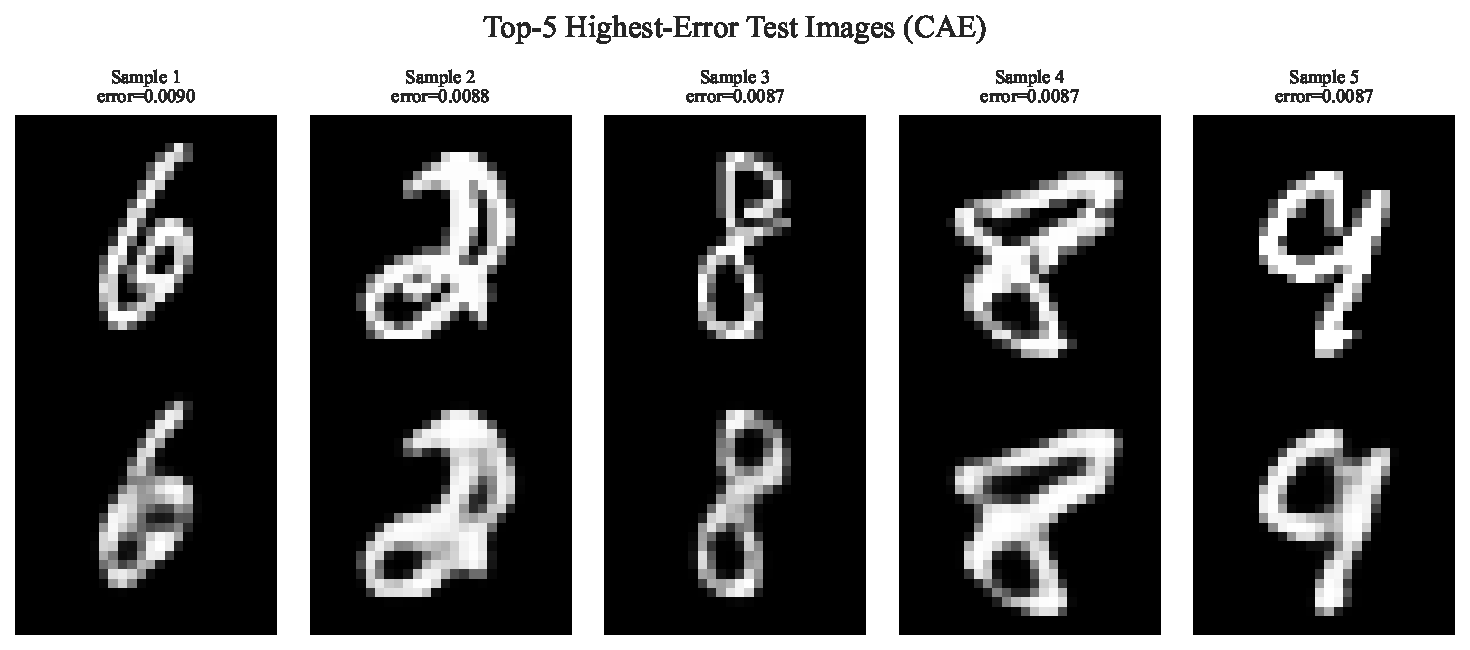
\includegraphics[width=0.6\linewidth]{Plot_Top5_HighError_Images}
\caption{The five test images with the largest CAE reconstruction error: originals (top) and reconstructions (bottom).}
\label{fig:top5}
\end{figure}

\subsection*{Why These Images Are Difficult}

The five errors are almost identical (0.0087 to 0.0090), so this group is just the
upper edge of the tail in Plot 9 and is not separated from the images below it.
Looking at the originals, sample 1 is a 6 whose tail loops back over the body, sample 2 is a scribbled 2 with thick
overlapping curves, sample 3 is an 8 written as two pieces with a gap,sample 4 is a very wide, tilted,
distorted 8 or 2, and sample 5 is a 9 with an irregular top loop and tail.

All of them are unusual, with odd slant, crossings, broken strokes or very thick
pen strokes. Such shapes are rare among the 10,000 training images, so the network
has learned less about how to encode them, and they carry more ink and more edges,
where a small misplacement is penalised.

%%%%%%%%%%%%%%%%%%%%%%%%%%%%%%%%%%%%%%%%%%%%%%%%%%%%%%%%%%%%
\section*{25. Consolidated Results}

\begin{center}
\begin{tabular}{|l|c|c|c|c|c|}
\hline
Model & MSE & MAE & SSIM & Parameters & Time\\
\hline
FC Autoencoder & 0.019970 & 0.054288 & 0.7735 & 211,040 & 16.14 s\\
Conv. Autoencoder & 0.002448 & 0.014828 & 0.9761 & 74,497 & 21.90 s\\
Denoising CAE & 0.004572 & 0.021277 & 0.9475 & 74,497 & 20.00 s\\
VAE & 0.053703 & 0.120811 & 0.3791 & 134,165 & 13.70 s\\
\hline
\end{tabular}
\end{center}

The values must be obtained from the student's own execution.

\subsection*{Reading the Consolidated Table}

Ranking by reconstruction quality gives: CAE (best), Denoising CAE, FC
autoencoder, VAE (worst), and the ranking is the same for MSE, MAE and SSIM.
There is no metric on which the models trade places, which is a useful
consistency check.

The number of parameters does not track quality. The CAE has the fewest
parameters of the reconstruction models and the best score, while the FC
autoencoder has the most and is second to last. What matters is whether the
architecture suits the data, and images have local spatial structure that
convolution uses well.

The timing column should be read loosely: these are single runs on Colab hardware
and include start-up cost in the first epoch (6--9 s of a 14--22 s total), so
differences of a few seconds are not a reliable ranking of speed.

%%%%%%%%%%%%%%%%%%%%%%%%%%%%%%%%%%%%%%%%%%%%%%%%%%%%%%%%%%%%
\section*{26. Required Inferences}

For every major plot, students must write a short inference containing:

\begin{enumerate}
\item What does the plot show?
\item What trend is observed?
\item Why might the observed trend occur?
\item What conclusion can be drawn?
\end{enumerate}

The following inferences are mandatory:

\begin{itemize}
\item effect of latent dimension on reconstruction;
\item difference between fully connected and convolutional reconstruction;
\item effect of Gaussian noise level;
\item ability of the denoising autoencoder to recover image structure;
\item characteristics of the VAE latent distribution;
\item structure of the two-dimensional VAE latent space;
\item quality and diversity of generated samples;
\item smoothness of latent-space interpolation;
\item relationship between reconstruction error and visual quality; and
\item differences between deterministic and probabilistic latent representations.
\end{itemize}

\subsection*{Inferences on the Mandatory Topics}

\textbf{1. Latent dimension.} In the FC-AE the test MSE fell from 0.0572 ($d_z=2$)
to 0.0321 (8), 0.0218 (16) and 0.0205 (32), and SSIM rose from 0.337 to 0.764
(Plot 10). A narrow code cannot store enough information, and the gains shrink
once the code can hold the main stroke information.

\textbf{2. Fully connected against convolutional.} The CAE had an 8.2 times lower
MSE and an SSIM of 0.976 against 0.774 (Plot 3). Convolutions keep neighbourhood
structure and share weights. Part of the gap is the CAE's larger bottleneck, and
at matched code sizes it is about twice as good in MSE.

\textbf{3. Gaussian noise level.} From $\sigma=0.1$ to 0.3 the MSE roughly doubles
(0.0036 to 0.0070) and SSIM falls from 0.962 to 0.882 (Plot 5). More noise hides
more of the stroke, and at $\sigma=0.3$ it is comparable with the thinner strokes.

\textbf{4. Recovering image structure.} In Plot 4 the output has a clean
background and continuous strokes, and all ten digits stay readable. With a
clean target the network learns digit shape and treats noise as something to
remove, so only fine detail is lost.

\textbf{5. VAE latent distribution.} The mean KL from the prior is only 3.4 nats
for the 2D VAE (10.7 for the 8D one), and the encoded means lie along a narrow
band and not over the whole prior (Plot 6). The KL term limits how much
information the code carries, and the 2D model mostly uses one dimension.

\textbf{6. Two-dimensional latent structure.} Digits 0 and 1 are separated at
opposite ends of the band, while 2--9 overlap in the middle. Two dimensions leave
too little room for ten classes, and similar digits (3/5/8, 4/7/9) compete for
the same region.

\textbf{7. Generated samples.} They look like blurred digits but are dominated by
a few classes (0, 9 and a 5/3/6-like blob), and several classes never appear
(Plot 7, Section 29.7). Random points decode only to the few shapes that occupy
the compressed latent space.

\textbf{8. Interpolation.} The 0-to-1 path changes without jumps but passes through
other digits (Plot 8), and the 3-to-8 path hardly changes at all (Section 29.8).
Smoothness comes from the KL term and the continuous decoder, but what the
in-between images look like depends on how well the classes are organised.

\textbf{9. Error against visual quality.} Low-error digits (the 7s in Plot 1,
$e\approx0.005$) look almost perfect, while high-error ones are blurred or change
shape (the 5 with $e=0.065$, the 3 that became an 8). Squared error follows
visual quality reasonably well within one model, although SSIM penalises blur more.

\textbf{10. Deterministic against probabilistic latent.} The AE and CAE map each
image to a point and reconstruct well (SSIM 0.77 and 0.98), but give no guarantee
of a smooth space that can be sampled. The VAE maps each image to a distribution,
so sampling and interpolation work, at the cost of much worse reconstruction
(SSIM 0.38 at $d_z=2$).

%%%%%%%%%%%%%%%%%%%%%%%%%%%%%%%%%%%%%%%%%%%%%%%%%%%%%%%%%%%%
\section*{27. Additional Latent-Dimension Study}

Repeat the basic autoencoder using:

\[
d_z\in\{2,8,16,32\}.
\]

Report:

\begin{center}
\begin{tabular}{|c|c|c|c|}
\hline
Latent Dimension & MSE & SSIM & Parameters\\
\hline
2 & 0.057150 & 0.3372 & 210,130\\
8 & 0.032065 & 0.6537 & 210,520\\
16 & 0.021826 & 0.7550 & 211,040\\
32 & 0.020513 & 0.7642 & 212,080\\
\hline
\end{tabular}
\end{center}

\textbf{Plot 10: Latent Dimension vs. Reconstruction MSE}

Students should explain the trade-off between compression and reconstruction
quality.

\begin{figure}[!htb]
\centering
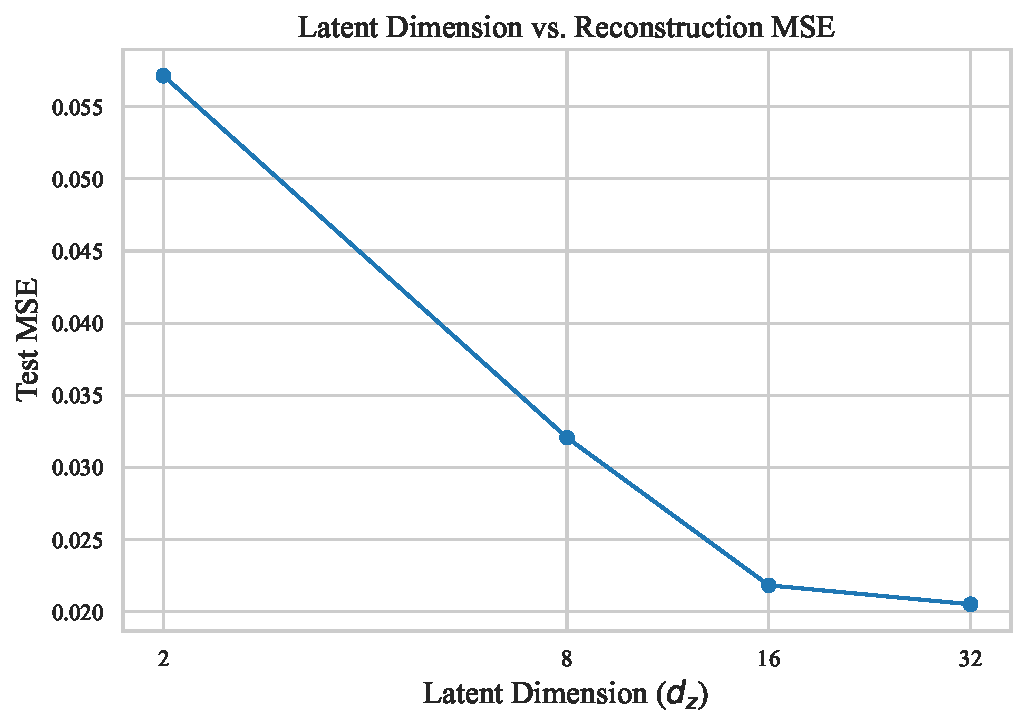
\includegraphics[width=0.5\linewidth]{Plot10_LatentDim_vs_MSE}
\caption{Plot 10: test MSE of the fully connected autoencoder against latent dimension (log$_2$ scale on the horizontal axis).}
\label{fig:plot10}
\end{figure}

\subsection*{Inference from Plot 10}

\textbf{The trend.} The MSE decreases at every increase of the latent dimension
but by less each time .SSIM follows the same pattern (0.337, 0.654, 0.755, 0.764).

\textbf{Why.} The parameter count barely changes (210,130 to 212,080, under 1\%),
so the differences come from the width of the bottleneck and not from model size.
Two numbers cannot carry the position, thickness and shape of a digit, so the
output is close to an average digit. Once the code is wide enough for the main
variations of MNIST (slant, thickness, identity), extra dimensions add little.

%%%%%%%%%%%%%%%%%%%%%%%%%%%%%%%%%%%%%%%%%%%%%%%%%%%%%%%%%%%%
\section*{28. Discussion Questions}

\begin{enumerate}
\item \textbf{What is an autoencoder?} A network trained to reproduce its own input, made of an encoder that
compresses the input and a decoder that rebuilds it.
\item \textbf{What is the purpose of the encoder?} To map the image to a compact latent representation that keeps its most important information.
\item \textbf{What is the purpose of the decoder?} To reconstruct the image from the latent representation. In a VAE it is also the generator for new images.
\item \textbf{What is a latent representation?} A learned, lower-dimensional description of the input: here the 16-number code, the feature map or the two-number VAE code.
\item \textbf{Why is the latent representation usually smaller than the input?} A code as large as the input lets the network copy without learning; a smaller one forces it to keep the essential structure.
\item \textbf{What happens when the latent dimension is too small?} Information is lost
and the reconstructions turn into blurred averages. At $d_z=2$ the FC-AE had an MSE of
0.0572 and an SSIM of 0.337.
\item \textbf{What happens when the latent dimension is increased?} The reconstruction
improves, with diminishing returns: the MSE was 0.0321, 0.0218 and 0.0205 at
$d_z=8$, 16 and 32. The code is also less compact and harder to visualise.
\item \textbf{Why can a convolutional autoencoder preserve spatial information more
effectively?} Convolutions work on local neighbourhoods with shared filters, so the 2D
layout of the image is kept in the feature maps. Flattening for a dense layer removes it.
\item \textbf{Differentiate an autoencoder and a denoising autoencoder.} A plain autoencoder reconstructs the clean image it receives; a denoising one receives a corrupted image and outputs the clean original.
\item \textbf{Why is the clean image used as the target in denoising?} With a noisy target the network would learn to reproduce the noise; with the clean target the loss rewards removing it.
\item \textbf{What happens when the noise level is increased?} MSE and MAE go up and SSIM
goes down (SSIM 0.962, 0.948, 0.882 for $\sigma=0.1,0.2,0.3$), and the drop is faster at high noise.
\item \textbf{Why are MSE, MAE and SSIM useful for image reconstruction?} MSE and MAE
measure the pixel-wise difference (MSE punishes large errors more), and SSIM compares
local structure, contrast and luminance, which is closer to how a person sees a blurred
image. Together they give a fuller picture than any one of them.
\item \textbf{What is a Variational Autoencoder?} An autoencoder whose encoder outputs a
probability distribution over $z$ (a mean and a variance), trained to reconstruct the input
while keeping this distribution close to a prior.
\item \textbf{How does a VAE differ from a conventional autoencoder?} The AE encodes each
image to a single point and is trained only on reconstruction. A VAE encodes it to a distribution,
samples from it, and adds a KL term to the loss.
\item \textbf{Why does a VAE learn a distribution instead of a single latent vector?} So
that nearby points in the latent space decode to similar images and the whole space is
covered smoothly, which is needed to sample new images from it.
\item \textbf{What is the reparameterization trick?} Writing the sample as
$z=\mu+\sigma\odot\epsilon$ with $\epsilon\sim\mathcal{N}(0,I)$, so that randomness comes from
$\epsilon$ and gradients can flow through $\mu$ and $\sigma$.
\item \textbf{Why is $\epsilon$ sampled from a standard normal distribution?} It is a fixed, parameter-free noise source, and scaling by $\sigma$ and shifting by $\mu$ gives an exact sample from $\mathcal{N}(\mu,\sigma^2)$.
\item \textbf{What is the role of KL divergence in the VAE loss?} It penalises the
encoder distribution for moving away from the prior $\mathcal{N}(0,I)$. This keeps
the latent space compact and continuous so that sampling works.
\item \textbf{What is the prior distribution used in the VAE?} A standard normal distribution,
$p(z)=\mathcal{N}(0,I)$.
\item \textbf{Why is a two-dimensional latent space useful for visualisation?} It can be
plotted directly as a scatter plot (Plot 6), so the structure of the codes can be seen without
any extra dimensionality reduction. The cost is a large loss in reconstruction quality.
\item \textbf{What does latent-space interpolation demonstrate?} Whether the latent space is
continuous. Smoothly changing decoded images along a line between two codes show that
the decoder maps nearby points to similar images.
\item \textbf{Why can a VAE generate new images?} Because the KL term makes the latent
codes follow roughly the prior, points sampled from that prior decode to plausible images.
\item \textbf{Why might some VAE-generated images be unclear?} Samples can land in
overlapping or empty regions of the latent space, the decoder averages the digits it associates
with a region, and the small code, sampling noise and short training all add blur.
\item \textbf{What is the difference between reconstruction and generation?} Reconstruction encodes
a real image and decodes it back. Generation starts from a sampled latent vector with no input
image at all.
\item \textbf{Why should test images remain unseen during training?} Otherwise the results measure memorisation and not generalisation. Here the test images were used only to monitor the validation loss, never to update weights or select models.
\end{enumerate}

%%%%%%%%%%%%%%%%%%%%%%%%%%%%%%%%%%%%%%%%%%%%%%%%%%%%%%%%%%%%
\section*{29. Additional Exercises}

\begin{enumerate}
\item Train the convolutional autoencoder with latent dimensions of 4, 8, 16
and 32 and compare reconstruction quality.
\item Compare Gaussian noise and salt-and-pepper noise using the same denoising
architecture.
\item Train the denoising autoencoder using two different noise levels and
compare SSIM.
\item Replace the convolutional decoder with transposed convolutions and
compare the reconstructions.
\item Implement a VAE with latent dimension 2 and 8 and compare the latent
representations.
\item Investigate the effect of increasing the KL-loss contribution.
\item Generate a larger grid of VAE samples and discuss diversity.
\item Select two digit regions in the latent space and perform interpolation.
\end{enumerate}

\subsection*{29.1 Convolutional Autoencoder with Latent Dimensions 4, 8, 16 and 32}

The base CAE has no scalar latent size, so a bottleneck was added between the
same convolutional stacks: Flatten $\rightarrow$ Dense($d_z$) $\rightarrow$
Dense($7\cdot7\cdot64$) $\rightarrow$ Reshape.

\begin{center}
\begin{tabular}{|c|c|c|c|c|}
\hline
$d_z$ & MSE & MAE & SSIM & Parameters\\
\hline
4 & 0.048396 & 0.109391 & 0.4698 & 65,797\\
8 & 0.024433 & 0.063071 & 0.7370 & 90,889\\
16 & 0.012034 & 0.037309 & 0.8732 & 141,073\\
32 & 0.009466 & 0.031895 & 0.9014 & 241,441\\
\hline
\end{tabular}
\end{center}

The same trade-off appears as for the FC model: the MSE roughly halves at each
step from 4 to 16 and improves by a further 21\% from 16 to 32. At equal latent
size the CAE is always better than the FC-AE of Section 27 (MSE 0.0244 against
0.0321 at $d_z=8$, 0.0120 against 0.0218 at 16, 0.0095 against 0.0205 at 32), and
its advantage grows from 1.3 to 2.2 times as the code widens. With a very small
code the limit is the code itself, so convolution has little to add. The CAE
parameter count grows with $d_z$ (the dense layers scale with
$7\cdot7\cdot64\cdot d_z$), and at $d_z=32$ it has more parameters than the FC model.

\subsection*{29.2 Gaussian Noise against Salt-and-Pepper Noise}

The same denoising architecture was trained on salt-and-pepper noise with
$p=0.10$ and compared with the Gaussian model ($\sigma=0.2$).

\begin{center}
\begin{tabular}{|l|c|c|c|}
\hline
Noise type & MSE & MAE & SSIM\\
\hline
Gaussian ($\sigma=0.2$) & 0.004572 & 0.021277 & 0.9475\\
Salt-and-pepper ($p=0.1$) & 0.004659 & 0.020884 & 0.9487\\
\hline
\end{tabular}
\end{center}

The two are practically tied. Salt-and-pepper is a little better in MAE and SSIM
and a little worse in MSE, but the differences (about 2\% in MSE and MAE, 0.001
in SSIM) are too small to rank the two from a single run, and the two noise
levels are not equal in strength anyway. A plausible reading is that
salt-and-pepper leaves most pixels untouched, so most pixels are recovered almost
exactly (good for MAE and SSIM), while a missed extreme pixel is a large squared
error (bad for MSE). Either way, the same CAE handles both kinds of corruption well.

\subsection*{29.3 Denoising Autoencoder at Two Training Noise Levels}

Two more denoisers were trained and tested at the same $\sigma$. The SSIM was
0.9664 at $\sigma=0.1$ and 0.9211 at $\sigma=0.3$, so the lower noise level is
easier to undo, in line with Plot 5. More useful is the comparison with the
$\sigma=0.2$ model of Section 14: at $\sigma=0.1$ it scored 0.9616 against 0.9664
for the matched model ($+0.005$), and at $\sigma=0.3$ it scored 0.8819 against
0.9211 ($+0.039$). Training at the test noise level therefore helps a little at
low noise and a lot at high noise, and a model trained at moderate noise handles
milder noise well but not stronger noise. (The noise seeds differ, but the gap at
$\sigma=0.3$ is far larger than a seed effect.)

\subsection*{29.4 Transposed Convolution Decoder}

\begin{center}
\begin{tabular}{|l|c|c|c|c|}
\hline
Decoder & MSE & MAE & SSIM & Parameters\\
\hline
UpSampling2D + Conv2D (Section 10) & 0.002448 & 0.014828 & 0.9761 & 74,497\\
Conv2DTranspose & 0.002265 & 0.014226 & 0.9768 & 74,497\\
\hline
\end{tabular}
\end{center}

The transposed decoder came out marginally ahead (MSE 7.5\% lower, SSIM higher by
0.0007), and the reconstructions look almost the same by eye, with 74,497 parameters each. The gap comes from single runs and is smaller than the
run-to-run variation seen in Section 27, so neither decoder can be called better.
On a simple dataset like MNIST both are sufficient.

\subsection*{29.5 VAE with Latent Dimension 2 and 8}

\begin{center}
\begin{tabular}{|c|c|c|c|c|}
\hline
$d_z$ & Rec. loss & KL loss & MSE & SSIM\\
\hline
2 & 172.913 & 3.448 & 0.053703 & 0.3791\\
8 & 129.539 & 10.658 & 0.035189 & 0.6340\\
\hline
\end{tabular}
\end{center}

With eight dimensions the reconstruction loss is 25\% lower, the MSE 34\% lower and
SSIM rises from 0.379 to 0.634, while the KL is about three times larger (10.7
against 3.4 nats), so the 8D code carries more information. The price is that the
space can no longer be shown on one scatter plot. The 8D VAE (MSE 0.0352) is still
worse than the plain 16-dimensional FC-AE (0.0200), so the regularisation and the
sampling noise cost accuracy as well.

\subsection*{29.6 Effect of Increasing the KL Contribution}

The KL term was multiplied by 5 in the training loss.

\begin{center}
\begin{tabular}{|c|c|c|c|c|}
\hline
KL weight & Rec. loss & KL loss & MSE & SSIM\\
\hline
1 & 172.913 & 3.448 & 0.053703 & 0.3791\\
5 & 161.434 & 3.087 & 0.048982 & 0.4538\\
\hline
\end{tabular}
\end{center}

The KL loss went down as expected (3.45 to 3.09), so the distribution moved closer
to the prior. A
heavier KL weight is normally expected to make reconstruction worse, but here it
improved .

\subsection*{29.7 Larger Grid of VAE Samples}

\begin{figure}[!htb]
\centering
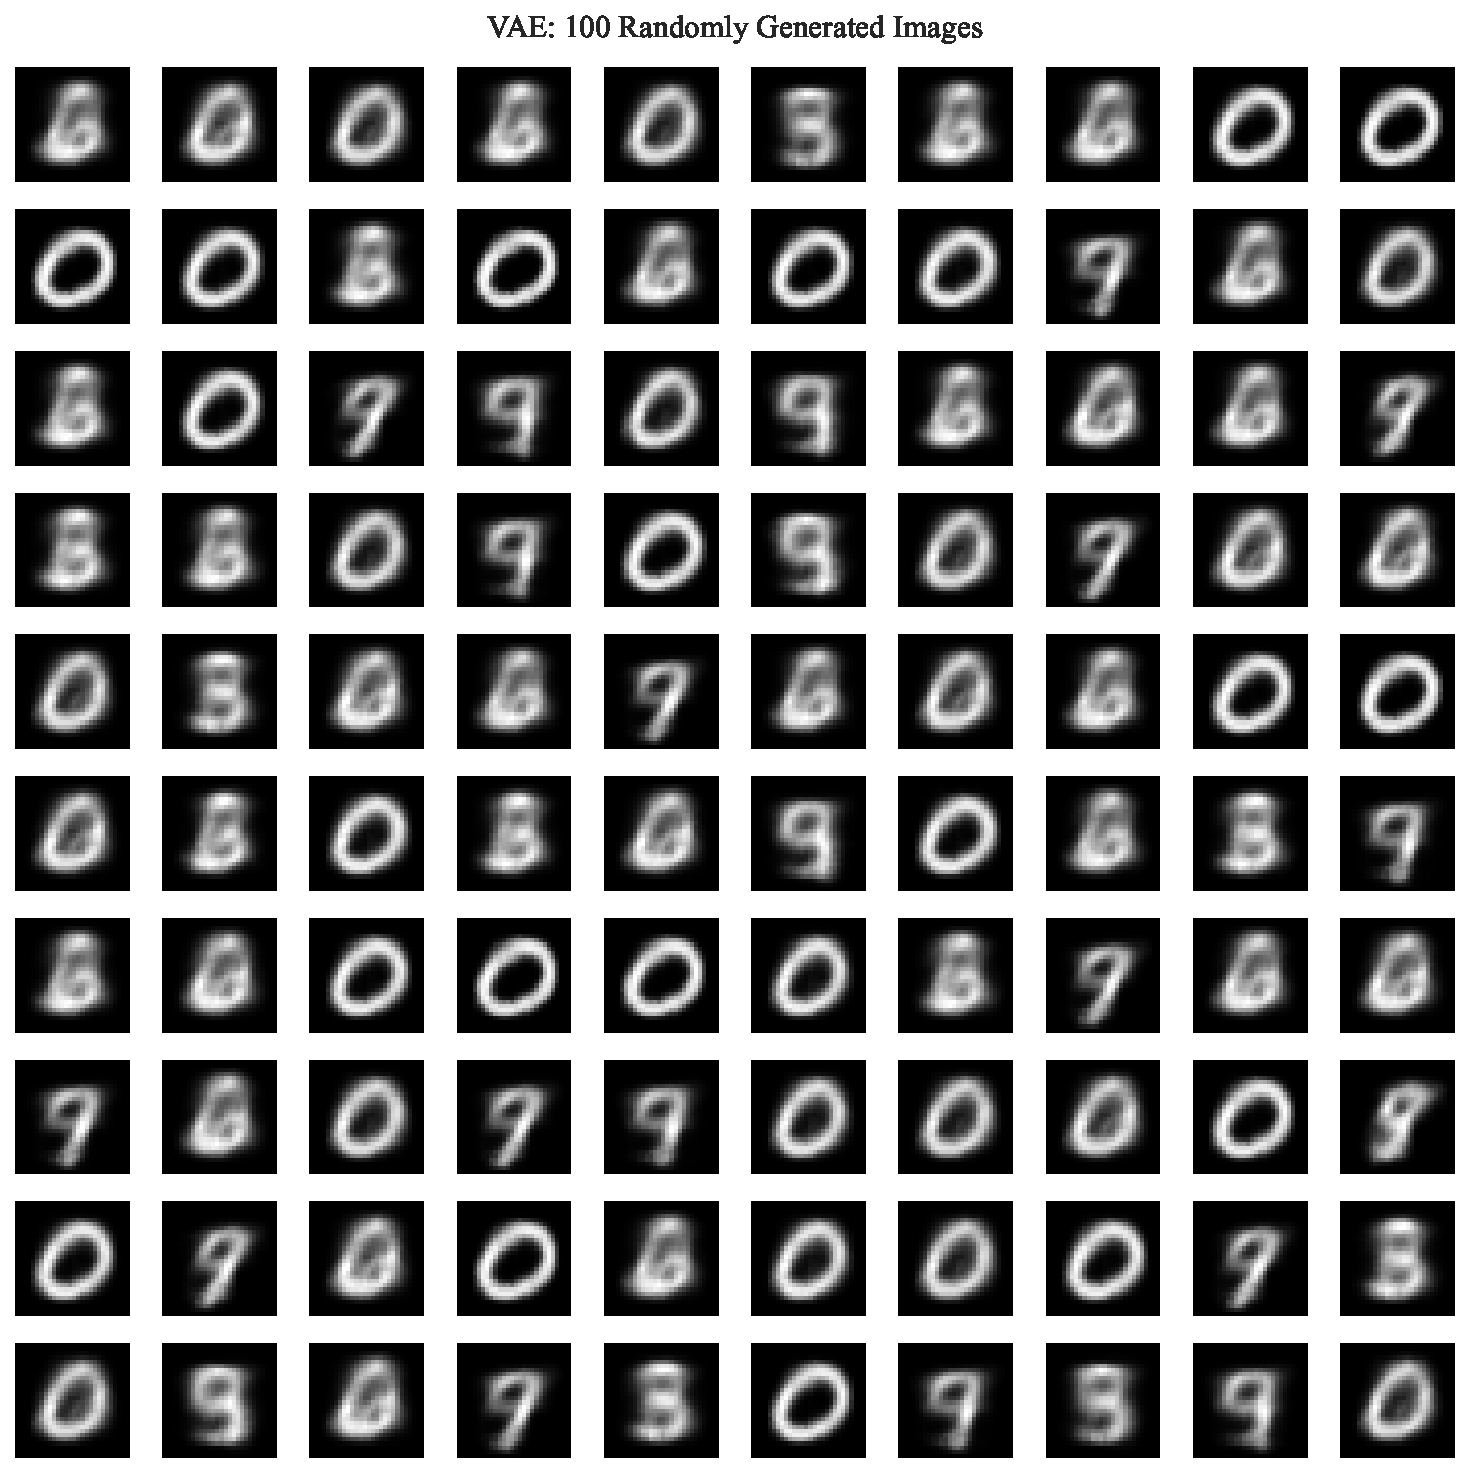
\includegraphics[width=0.46\linewidth]{Extra7_VAE_Large_Sample_Grid}
\caption{100 images generated from random points $z\sim\mathcal{N}(0,I)$.}
\label{fig:extra7}
\end{figure}

With 100 samples the low variety is easier to see. Three groups dominate: clean 0s
(the largest and sharpest group), slanted 9- or 7-like shapes, and blurry blobs
that could be a 5, 6 or 8. There is hardly any clear 1 and no clear 2, 3 or 4.
This matches Plot 6, where random points from the prior fall mostly at the 0
end of the band or in the crowded middle.

\subsection*{29.8 Interpolation between Two Digit Regions}

\begin{figure}[!htb]
\centering
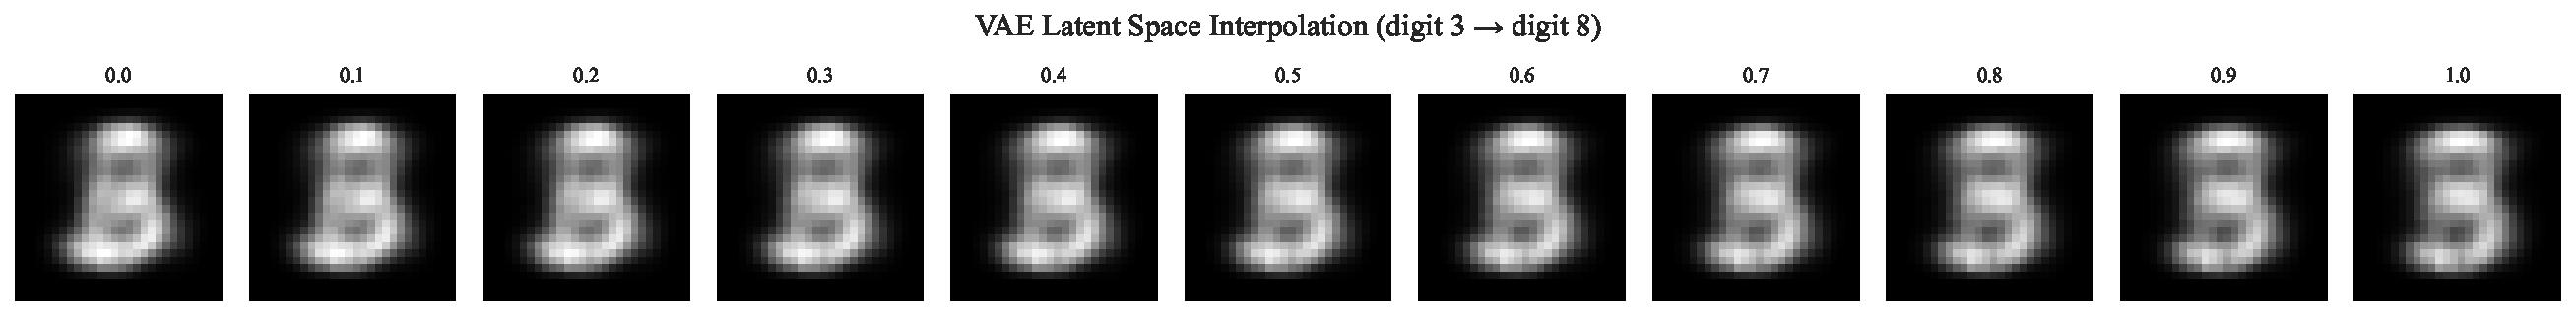
\includegraphics[width=0.86\linewidth]{Extra8_VAE_Interpolation_3_to_8}
\caption{Decoded images along the line between the latent means of a test 3 ($\alpha=0$) and a test 8 ($\alpha=1$).}
\label{fig:extra8}
\end{figure}

The 3-to-8 path behaves very differently from the 0-to-1 one. All eleven frames
look almost the same, a blurred stacked shape that could be a 3, 5 or 8. The path
is smooth but shows no morph, because 3 and 8 lie close together in the crowded
middle of Plot 6, so both endpoints decode to nearly the same image. This is
better evidence about the limit of a 2D latent space than a nicer-looking
interpolation would have been.

%%%%%%%%%%%%%%%%%%%%%%%%%%%%%%%%%%%%%%%%%%%%%%%%%%%%%%%%%%%%
\section*{30. Expected Outcome}

At the end of the experiment, students should be able to demonstrate the
complete image-representation and reconstruction pipeline:

\[
\boxed{
\text{Image}
\rightarrow
\text{Encoder}
\rightarrow
\text{Latent Representation}
\rightarrow
\text{Decoder}
\rightarrow
\text{Reconstructed Image}
}
\]

They should also demonstrate denoising:

\[
\boxed{
\text{Clean Image}
\rightarrow
\text{Noise}
\rightarrow
\text{Denoising Autoencoder}
\rightarrow
\text{Recovered Image}
}
\]

and variational generation:

\[
\boxed{
\text{Image}
\rightarrow
(\mu,\sigma)
\rightarrow
z
\rightarrow
\text{Decoder}
\rightarrow
\text{Generated/Reconstructed Image}
}
\]

The final report should contain both quantitative evaluation and visual
analysis. Numerical performance values must be obtained from the student's
own execution.

\subsection*{Conclusion}

All four models were built, trained and evaluated on a common MNIST set-up. The
fully connected autoencoder reconstructs the coarse layout of a digit from a
16-number code but blurs the fine detail (MSE 0.0200, SSIM 0.774). The
convolutional autoencoder is much better (MSE 0.0024, SSIM 0.976), partly because
convolution suits images and partly because its bottleneck is large. The denoising
CAE, trained with a clean target, removes Gaussian noise of $\sigma=0.2$ (SSIM
0.948) and still returns readable digits at $\sigma=0.3$ (SSIM 0.882). The
two-dimensional VAE reconstructs poorly (SSIM 0.379) but has a latent space
from which new, blurry, digit-like images can be drawn, and along which the
decoded image changes without jumps. The latent-dimension studies show the
same compression against quality trade-off for every model, with large gains
up to about 16 dimensions and little beyond.

\subsection*{Limitations}

\begin{itemize}
\item Every number comes from a single run with one seed. The FC-AE at
$d_z=16$ gave MSE values 9\% apart in two runs (Sections 9 and 27), so
differences of that size (the 16 to 32 latent step, the transposed against
up-sampling decoder, and the KL weight experiment) should not be treated as real.
\item The 2,000 test images were also used as the validation set, although they
were not used for model selection.
\item All models were trained for the same 20 epochs. The FC-AE and the VAE were
still improving at the end, so their results are somewhat pessimistic.
\item The CAE bottleneck of $7\times7\times64$ is larger than the input, which
makes the comparison in Section 11 favourable to the CAE.
\item The VAE metrics use a sampled $z$, and the VAE uses only two latent
dimensions and a 16-unit layer before the latent heads, so its poor
reconstruction cannot be blamed on the VAE idea alone.
\item The reconstruction quality of the noisy input itself was not computed, so the
gain of the denoiser is only shown visually.
\end{itemize}


%%%%%%%%%%%%%%%%%%%%%%%%%%%%%%%%%%%%%%%%%%%%%%%%%%%%%%%%%%%%
\section*{31. References}

\begin{enumerate}
\item Ian Goodfellow, Yoshua Bengio and Aaron Courville,
\emph{Deep Learning}, MIT Press, 2016.

\item Diederik P. Kingma and Max Welling,
``Auto-Encoding Variational Bayes,'' ICLR, 2014.

\item Pascal Vincent et al.,
``Stacked Denoising Autoencoders: Learning Useful Representations in a Deep
Network with a Local Denoising Criterion,'' Journal of Machine Learning
Research, 2010.

\item Yann LeCun, Corinna Cortes and Christopher J. C. Burges,
``MNIST Handwritten Digit Database.''

\item TensorFlow Documentation:
\url{https://www.tensorflow.org}

\item Keras Documentation:
\url{https://keras.io}

\item scikit-image Documentation:
\url{https://scikit-image.org}

\item Zhou Wang, Alan C. Bovik, Hamid R. Sheikh and Eero P. Simoncelli,
``Image Quality Assessment: From Error Visibility to Structural Similarity,''
IEEE Transactions on Image Processing, 2004.

\item Carl Doersch, ``Tutorial on Variational Autoencoders,'' arXiv:1606.05908, 2016.

\item Diederik P. Kingma and Jimmy Ba, ``Adam: A Method for Stochastic Optimization,''
ICLR, 2015.
\end{enumerate}

%%%%%%%%%%%%%%%%%%%%%%%%%%%%%%%%%%%%%%%%%%%%%%%%%%%%%%%%%%%%
\section*{32. Source Code}

The complete notebook, plots and report for this experiment are available at:

\url{https://github.com/smadhav2024/Deep_Learning_Lab/tree/main/Lab%207}

\end{document}
